% add. options: [seceqn,secthm,crcready]
\documentclass[sw]{iosart2x}
%\usepackage[T1]{fontenc}
\usepackage{cleveref}
\usepackage{csquotes}
\usepackage{aurl}
\usepackage{booktabs}
\usepackage{tabulary}
\usepackage{siunitx}
\usepackage{tablefootnote}
%\usepackage{dcolumn}
%\usepackage{placeins} %provides \FloatBarrier
\newcommand{\aw}{AnthroWorks3D}
\newcommand{\anno}[1]{\href{https://annosaxfdm.de/ontology/#1}{\texttt{#1}}}
\newcommand{\gfo}[1]{\href{https://www.onto-med.de/ontologies/gfo/#1}{\texttt{#1}}}
\newcommand{\fma}[1]{\href{http://purl.org/sig/ont/fma/fma#1}{\texttt{#1}}}
\newcommand{\latin}[1]{\emph{#1}}
\daurl{anno}{https://annosaxfdm.de/ontology/}
\daurl{gfo}{https://www.onto-med.de/ontologies/gfo\#}
\daurl{fma}{http://purl.org/sig/ont/fma/fma}
\daurl{ta2}{https://ta2viewer.openanatomy.org/?id=}

\pubyear{2023}
\volume{0}
\firstpage{1}
\lastpage{1}

%\overfullrule=10pt % for debugging overfull hboxes
\begin{document}

\begin{frontmatter}

%\pretitle{}
\title{The ANthropological Notation Ontology (ANNO): A core ontology for annotating human bones and deriving phenotypes}
\runtitle{Anthropological Notation Ontology}
%\subtitle{}

\begin{aug}
\author[B,C]{\inits{M.}\fnms{Marie} \snm{Heuschkel}\ead[label=e2]{marie.heuschkel@hs-mittweida.de}}
\author[A,C]{\inits{K.}\fnms{Konrad} \snm{Höffner}\ead[label=e1]{konrad.hoeffner@uni-leipzig.de}%
\thanks{Corresponding author. \printead{e1}.}
}
\author[B]{\inits{F.}\fnms{Fabian} \snm{Schmiedel}\ead[label=e3]{fabian.schmiedel@hs-mittweida.de}}
\author[B]{\inits{D.}\fnms{Dirk} \snm{Labudde}\ead[label=e10]{dirk.labudde@hs-mittweida.de}}
\author[A]{\inits{A.}\fnms{Alexandr} \snm{Uciteli}\ead[label=e11]{alexandr.uciteli@imise.uni-leipzig.de}}
\address[A]{Institute for Medical Informatics, Statistics and Epidemiology (IMISE), \orgname{Leipzig University},
Saxony, \cny{Germany}\printead[presep={\\}]{e1,e11}}
\address[B]{\orgname{Hochschule Mittweida},
Saxony, \cny{Germany}\printead[presep={\\}]{e2,e3,e10}}
\address[C]{equal contribution}
\end{aug}

\begin{abstract}
The Anthropological Notation Ontology (ANNO) allows the systematic and standardized classification of recovered bone finds into the skeletal system, the description of the skeletal pieces, and the definition of functions for deriving different phenotypes of humans in forensic and historical anthropology.
ANNO consists of two components:
ANNOdc, a domain-core ontology providing core entities such as basic anatomical categories, and ANNOds, a domain-specific ontology used for annotating structures of the human skeleton.
ANNO is integrated into AnthroWorks3D, a photogrammetry pipeline and application for the creation and analysis of 3D-models of human skeletal remains.
The integration is based on the three-ontology method with the General Formal Ontology as the top-level ontology, ANNOdc as the task ontology and ANNOds as the domain ontology.
Thus, AnthroWorks3D only needs to implement access to the entities (classes and properties) of the task ontology, whereas the entities of the corresponding domain ontology are imported dynamically.
ANNO supports the analysis of skeletal and bone finds in forensic and historical anthropology, facilitating the standardization of data annotation and ensuring accurate preservation of information for posterity.
\end{abstract}

\begin{keyword}
\kwd{Ontology}
\kwd{Ontology development}
\kwd{Anthropology}
\end{keyword}

\end{frontmatter}

\section{Introduction}\label{sec:introduction}

Anthropology, as a discipline, explores the full range of human diversity and similarity across cultures, social structures, habitats and environments.
Anthropological skeletal analysis, a subset of this field, is particularly focused on understanding the human skeletal system.
This study encompasses a multidisciplinary approach, integrating insights from natural, social and cultural sciences.

It's about reading the stories that human remains tell---from sex, age and health to broader aspects like cultural practices and environmental impacts.
Hence, data from historical and prehistoric anthropology~\cite{prehistoricanthropology}, as well as modern forensic science, provides a comprehensive understanding of deceased individuals and past populations from different time periods.
This process involves investigating individuals' identity, health status, behavior, lifestyle, culture, and the circumstances of their death~\cite{spurensuche} by determining phenotypes such as sex, age, height, ancestry, and other individualizing traits using anthropological methods.
Sex assessment is a key part of this analysis because it provides essential information about an individual's identity and helps build a biological profile.
This profile offers insights into the person's life, health, and the population they belonged to, aiding in reconstructing past societies, understanding demographic patterns, and identifying individuals in forensic cases.

The Anthropological Notation Ontology (ANNO) is motivated by the need for consistent data recording, enhanced comparability, facilitated access to, and sustainable preservation of human skeletal remains for research and cultural heritage contexts.
It provides a standardized, digital framework for documenting, analyzing, and presenting data from human skeletal remains, making information accessible and usable for future research.
ANNO supports the use of digital 3D models of bones in 3D editors such as AnthroWorks3D, playing a crucial role in categorizing and analyzing data in a flexible yet standardized and machine-readable manner, thus ensuring interoperability across different systems and studies.
Anthropological analysis of human skeletal remains is inherently comparative, heavily relying on reference collections \citep{spurensuche}.
Several key challenges profoundly affect anthropological research \citep{aw3dcidoc}:

\paragraph{Preservation}\label{sec:preserve}
From the moment of excavation, skeletal remains are subject to wear and tear, diminishing their informational value.
Transferring the examination to digital models reduces physical handling, minimizes deterioration, and ensures that data is preserved and accessible for future research, even in cases of repatriation or reburial.
This is crucial because "knowledge and evidence production can only yield what the original material provides."~\cite[p.~132]{HeuschkelSchmiedelLabudde2024}
Exemplifying ANNO's underlying utility in this regard is the Rödelheim skeletal collection curated and researched by the Department of Historical Anthropology and Human Ecology at the University of Göttingen, consisting of over 200 skeletal remains from Napoleon's army.
With these remains scheduled for reburial in 2021, digitization became essential.
For instance, by creating digital 3D models via AnthroWorks3D, and annotating them based on the ANNO ontological framework, the models were converted into research data that is analyzable across studies, despite the physical remains being reburied.

\paragraph{Access}\label{sec:access}
Anthropological skeletal material from excavations often remains undetermined due to a shortage of specialists at the respective institutions.
A digital solution would provide greater availability of human skeletal remains and allow for the efficient allocation of anthropologists and collections.
For example, the Archaeological Heritage Office of Saxony faces a significant backlog of unevaluated skeletal collections due to a shortage of anthropologists.
For instance, by digitizing these remains and using ANNO for annotation, the data can be made available to experts worldwide.
This approach allows for the efficient allocation of resources, enabling comprehensive analysis that would otherwise be infeasible.

\paragraph{Comparability and Transparent Documentation and Analysis}\label{sec:comp+transp} 
Existing data recording systems in anthropology are often individualized, leading to compatibility issues that hinder comparative analysis and comprehensive intra- and interdisciplinary research~\cite{HeuschkelSchmiedelLabudde2024}.
A digital solution combining ANNO, a standardized ontology for skeletal data, and AnthroWorks 3D, a 3D editor for creating and annotating digital bone models, provides unprocessed and undistorted information, making it comprehensible, reproducible, and sustainably documented.
It also supports flexible and objective documentation of bone parts or fragments~\cite{aw3dcidoc}.
This allows researchers to "surround themselves with every shred of information about a collection or an object,"~\cite[p.~148]{Palkovich.2001} with future possibilities such as integration into collection management systems and the application of AI analysis \cite{HeuschkelSchmiedelLabudde2024}. 
For instance, researchers comparing skeletal remains from different regions can use ANNO to standardize their annotations, ensuring that data from disparate sources is compatible.
For instance, if two teams are studying bone wear patterns to infer lifestyle differences using different skeletal collections, ANNO allows them to document their findings in a uniform manner, facilitating direct comparisons and more robust conclusions.

While the concept of ANNO encompasses a broad range of anthropological aspects, its first and fundamental module, which is the focus of this paper, is on skeletal anatomy.
This module serves as the foundation for all subsequent developments within the ANNO framework.

In anthropological skeletal analyses, methods employed include morphological and osteometric examinations.
Apart from contextual information, anthropological focus on identifying and analysing traces found directly on the bones, indicating bone reactions or functional aspects.

For this purpose, anthropologists use human anatomy, specifically the skeletal system and further tissues of the musculoskeletal system, to classify and describe and thus document bones, anatomical structures, and diagnostic features within the overall framework of the skeleton in a comprehensive and transparent fashion.
Precisely locating the traces on the skeleton is crucial.
Accurate identification and mapping of these features allow for a detailed understanding of their implications and connections to broader anthropological inquiries.
This precision is vital for meaningful and reliable interpretations in anthropological research.
By applying the same principles used for mapping the Earth's surface \enquote{terrain}, a detailed map of the human body can be created.
This map contains visible anatomical surface structures, as well as artificial objects such as measurement points or content-related or methodologically based classifications and boundaries~\citep{topo}.
ANNO represents such a map by providing an ontology for accurate and exhaustive definitions that allow to unequivocally locate these, facilitate their retrieval and furthermore serve as a basis for an objective examination, including measurements.


Osteometric examinations involve precise measurements that numerically capture features important in anthropology.
These measurements are crucial for discriminant function analysis, a key method for determining the biological sex of deceased individuals.
Discriminant function analysis identifies differences between predefined groups, such as males and females, by assessing specific bone measurements that typically differ between the sexes, such as the size and shape of certain features.
The goal is to pinpoint characteristics that significantly differentiate these groups.
The resulting discriminant function includes measurements as variables and their weights representing these characteristics.
By inputting these measurements into the formula, the discriminant function calculates a score that classifies skeletal remains into one of the groups, indicating the likelihood of the remains being male or female~\citep{prehistoricanthropology} .


The digitization and digitalization of anthropological skeletal materials offer significant advantages.
This process extends beyond visualizing remains to creating and analyzing annotated 3D models, incorporating traditional anthropological methods into digital formats.
Such technological advancements facilitate preservation, documentation, and global collaboration, allowing remote access and minimizing physical specimen wear.
These developments address access challenges and enable the linking of diverse study samples, thus enhancing research and data integration.
The digital 3D models can serve as digital twins, as they present virtual, detailed replicas of skeletal remains, created using 3D imaging technologies.
ANNO complements this digital twin by providing an ontological framework that enriches the model with detailed, accurate anthropological data.
This synergy enhances the digital twin's utility, enabling precise annotation, analysis, and sharing of anthropological findings.
The benefits include improved research efficiency, enhanced data sharing and collaboration opportunities, and a deeper, more nuanced understanding of anthropological subjects.
It provides a consistent yet flexible framework for representing anthropologically relevant anatomical and anthropological knowledge.
By mapping information directly onto 3D models, ANNO ensures that data is not only comprehensible and reproducible but also sustainably documented.
This approach improves data interoperability, a crucial prerequisite for successful digitization.
Furthermore, data sets consolidated this way and formalized through the Anthropological Notation Ontology (ANNO) presented here allow for efficient data analysis techniques, such as data and text mining that promote deeper insights.
Therefore, the contribution of ANNO lies in its ability to encapsulate and connect anthropological methods, aspects, and skeletal features within an ontological structure that aids in the digitization process, promoting more in-depth anthropological research and broader interdisciplinary studies.

%\paragraph{Theoretical Background}
% KH: Prepended this paragraph with "Generally" for a slightly better tie-in to the one before. Everyone feel free to improve if you find a better way.
Generally, ontologies are theories about the kinds of objects, the properties of objects, and the relations between objects in a knowledge domain.
On the one hand, these are controlled vocabularies, but on the other hand, ontologies are also conceptualizations that the vocabulary terms are intended to capture~\citep{whatareontologies}.
Researchers in many areas recognized the need for ontologies to clearly define specialized vocabularies for these domains~\citep{evaluatingdomain}.
The success of using ontologies to annotate biological data can also be confirmed by multiple examples~\citep{biomedicalontologies}.
It was therefore an easy decision for us to use an ontology for modeling the anthropological domain.

%\paragraph{Tasks}
The main tasks to be supported by the intended ontology are the annotation of anthropological models, the specification of spatial relations between anatomical entities and the definition of phenotyping functions, see \cref{sec:methodology}.
However, the ontology must remain relatively simple and compact to allow easy handling by domain experts and efficient integration into software.
Existing anatomical ontologies often lack standardization in the naming and definition of concepts.
Furthermore, the hierarchical structure is often too complex or general to be efficiently integrated into software for realizing specific anthropological use cases, see \cref{sec:otherontologies}.
Since we could not find any ontologies that fully met our requirements and the integration or adaptation of selected ontology parts would be much more complex, we decided to develop a new ontology and then map it to the most prominent one.

\begin{table}[h]
\centering
\caption{Structure, properties and publication of ANNO.}
\label{tab:publication}
\begin{tabular}{ll}
\toprule
%Property			&Value\\
%\midrule
Modules				&ANNOdc (domain-core), ANNOds (domain-specific)\\
Top-Level Ontology	&General Formal Ontology~\citep{gfo}\\
Namespace			&\url{https://annosaxfdm.de/ontology/}\\
%Browser			&RickView~\citep{rickview} at \url{https://annosaxfdm.de/ontology/}\\
Browser				&RickView\tablefootnote{\url{https://github.com/KonradHoeffner/rickview}} at \url{https://annosaxfdm.de/ontology/}\\
Repository			&\url{https://github.com/annosaxfdm/ontology}\\
Terminology Server	&\url{https://ols.imise.uni-leipzig.de/ontologies/anno}\\
License				&\href{https://creativecommons.org/licenses/by/4.0/}{Creative Commons Attribution 4.0 International}\\
DOI (all versions)	&\href{https://doi.org/10.5281/zenodo.8301559}{10.5281/zenodo.8301559}\\
\bottomrule
\end{tabular}
\end{table}

%\paragraph{Main contributions}
% rest of old text
%ANNO consists of two components: ANNOdc, a domain-core ontology providing core entities such as basic anatomical concepts and classifications, and ANNOds, a domain-specific ontology employed for annotating human skeletal structures.
%
%new text:
Our main contributions are the following:
\begin{enumerate}
\item ANNOdc (\cref{sec:annodc}, \cref{fig:annodc}) is a domain-core (dc) ontology that defines the core entities of the domain.
This includes general anatomical categories (Bone and Tooth), a category for describing their characteristics (Anatomical property), anatomical spatial entities (Anatomical space, surface, line and point) as well as the category Phenotype to model the rules for determining human phenotypes.
ANNOdc was embedded in the General Formal Ontology (GFO), i.e. the ANNOdc classes are subclasses of GFO classes.
%
\item ANNOds (\cref{sec:annods}) is a domain-specific (ds) ontology for describing domain-specific entities to be used for annotating the parts of the human skeleton.
These are bones, teeth, their parts and compounds, such as mandible, Mental protuberance or the facial skeleton.
It is also used for modeling their properties and relations, such as the distance between \latin{Mentale dexterum} and \latin{Mentale sinistrum}, needed to derive human phenotypes like sex or height.
ANNOds is embedded in ANNOdc.
In its current version, the ontology refers to standardized normal adult anatomy, excluding developmental aspects, variations, pathologies and other related factors.
%
\item ANNO is integrated into \aw{} (\cref{sec:aw}), a photogrammetry pipeline and application for generating and analyzing 3D-models of human skeletal remains.
%
\item ANNO is published over multiple channels, see~\cref{tab:publication}.
%
\end{enumerate}

The intended audience for the Anthropological Notation Ontology encompasses all anthropologists and professionals working in related settings, including museums and archaeological contexts.
This audience is critical as the digitization of skeletal remains and the development of comprehensive data management systems are essential advancements for the sustainability of the discipline.
Over the past decade, there has been a growing recognition of the importance of digital transformation in anthropology, which is crucial for the long-term preservation, accessibility, and analysis of anthropological data.

ANNO plays a pivotal role in this digital transformation as it represents a significant step in this digitalization effort, serving as a bridge between various fields such as IT, semantic web technologies, ontology development, and anthropology.
By creating a unified platform for the digitization, annotation, and analysis of skeletal remains, ANNO not only enhances the efficiency and accuracy of anthropological research but also fosters interdisciplinary collaboration.
This collaboration is vital for addressing the complex challenges in the field and ensuring that the methodologies and findings in anthropology remain robust and relevant in the digital age.

Tools such as ANNO and AnthroWorks 3D are the driving forces and bridges of digitization, enabling the much-needed digital transformation in anthropological research.
They provide a comprehensive and sustainable solution, enhancing our understanding of human history and cultural heritage.

\section{State of research}\label{sec:stateofresearch}

\subsection{Distinguishing features of the Anthropological Notation Ontology}\label{sec:distinguishingAnno}
ANNO distinguishes itself by focusing specifically on anthropology rather than general anatomy.
This focus underscores the importance of understanding the relationship between bones and the anatomical and osteometric features found on them.
ANNO emphasizes the need for precise definitions using established anatomical and anthropological terminology, including directional terms, to facilitate clear communication within the field.
This approach allows for a more nuanced understanding of human skeletal structures, essential for anthropological analysis and research.
The ontology aims to map the entirety of anthropological knowledge directly onto a digital 3D skeletal model, functioning as a comprehensive knowledge representation.
It projects anthropological information as a layer onto the skeleton, incorporating and localising aspects and interrelations crucial for anthropological study, effectively serving as a navigable atlas for skeletal analysis.

ANNO is designed to align anthropological knowledge, including measurement explanations and landmark identification, with methods and the skeletal framework itself.
This modeling ensures data compatibility for extensive analysis, integrating a maximal amount of information.
A pivotal advantage of ANNO is its ability to directly associate information with a digital 3D model facilitating the inherent connection to the raw data and enhancing comprehension, reproducibility, and sustainability of documentation.
ANNO meticulously details skeletal anatomy through an atomic design approach, breaking it down into its most basic, indivisible components, then systematically organizing these components to represent the skeletal structure with high fidelity.

This granular method facilitates a deep and scalable anthropological understanding.
ANNO is capable of referencing various (online) resources, even those that are structurally and semantically diverse, such as other terminologies, ontologies, websites~\citep{atinfo} or media, aiming for synonym mediation, standardisation and conceptual clarity.

The current state of ANNO includes a foundational module that focuses on skeletal anatomy on the one hand and anthropological aspects such as osteometric landmarks (measurement points) and measurements (distances),
which are either sporadically represented or absent in existing ontologies, on the other hand.
ANNO is designed to evolve gradually by integrating more anthropological aspects, ultimately becoming a modular knowledge environment.
This approach allows for step-by-step enhancements to the ontology's scope and utility, enabling a comprehensive integration of anthropological knowledge.

\subsection{Existing solutions and research gaps}\label{sec:Solutions+Gaps}
\paragraph{Nomenclatures: Terminologia anatomica (TA)}\label{sec:ta}
There are various reference materials for the description of anatomical structures, ranging from anatomical atlases to nomenclatures.
The latter aim for an established standardized naming and systematization.
The TA~\citep{ta2} is a hierarchy of anatomical structure concepts for the entire human body.
For historical reasons, it uses a terminology consisting of Latin and originally Greek, which was later latinized.
For each anatomical structure, the TA provides the \enquote{preferred}, i.e. standard, Latin term and its English equivalent as well as an individual identification number.
In some cases, Latin and English synonyms are also included, e.g. \emph{malar bone} is an English synonym of the Latin preferred term \latin{Os zygomaticum} and its English equivalent \emph{zygomatic bone}.
The identification number is crucial, as certain landmarks are mostly listed without bone affiliation, resulting in multiple occurrences. %(s. Bone Part)
For instance, the \latin{Processus zygomaticus} can be found both at the \latin{Os frontale} and the \latin{Os temporale}.
Eponyms are terms derived from proper nouns such as the name of a person, place or thing, and they are considered a type of synonyms since they stand for the same anatomical structure.
For example, \latin{Ossa digitorum manus / pedis} (engl. \emph{phalanges of the hand}, respectively \emph{foot}) are the small bones of the fingers and toes and are also denoted as \latin{Phalanges manus / pedis} which are named after the Greek word \emph{phalanx} for a dense rectangular infantry formation.
In addition to the outdated print edition~\citep{ta1998}, an extended second edition (TA2) is available online~\citep{ta2}.
Furthermore, there is a commercially available independent companion print publication with German~\citep{anatomylexicon}, English~\citep{pocketatlas} and Spanish~\citep{taspanish} editions of which at least the German edition is regularly updated.
This book contains textual and visual descriptions, whereby anatomical structures are indicated through lines on the illustrations.

\paragraph{Existing ontologies: Foundational Model of Anatomy (FMA)}\label{sec:OntologiesFMA}
Other ontologies either lack a comprehensive approach to anthropology or exhibit inconsistency in depicting knowledge within this field, since they are not designed with this specific purpose in mind.
The FMA~\citep{fma} ontology represents the physical organization of human anatomy by mapping relations to one another.
It allows the knowledge it contains to be represented in a way that is humanly comprehensible and machine-interpretable.
The FMA uses the Basic Formal Ontology (BFO) as its top-level ontology.
Corresponding to its relational nature, new higher level concepts are introduced and used for reorganizing the actual anatomical structures diverging from the TA's hierarchical structure.
Thus, in 90\,\% of the cases this leads to new creations of anatomical concepts~\citep{anatomicalterms} whereas only 1\,\% contain textual definitions~\citep{uberon}.
The FMA primarily focuses on depicting the entirety of human anatomy.
This broad approach results in inconsistencies in how skeletal structures are detailed, as the FMA's overarching goal to cover anatomy in general cannot sufficiently address the complexities and nuances of skeletal anatomy.
Such a wide scope also means that the anatomical knowledge pertaining to the skeleton is not depicted with the depth or precision that anthropological work demands, reflecting the limitations in existing literature on the subject.
From an anthropological perspective, the FMA ontology exhibits challenges in terms of content depth, comprehensiveness, and granularity.
Specifically, the main issues encompass a lack of cross-references between concepts, taxonomic and hierarchical inconsistencies, insufficient detail levels, and conceptual ambiguity.
These gaps result in a notable absence of detailed relationships, associations, and concepts that are crucial for a thorough anthropological understanding and analysis.
Additionally, the distinction between normal anatomy, pathology, and anatomical variants, which is essential, is not adequately addressed by the FMA's architecture.

The following examples illustrate the issues described above.

\begin{itemize}
\item Specific bones can be found as a subclass of \emph{bone organ} (\aurl{fma}{224804}) but, among others, also in terms of tissue as \emph{bone tissue} (\aurl{fma}{224804}) with then varying terms such as \emph{bone tissue of hip bone} (\aurl{fma}{42854}) or \emph{bone of sacrum} (\aurl{fma}{43624}) and placed on the same level as histological structures like \emph{lamellar bone} (\aurl{fma}{224806}).
\item Different anatomical landmarks are classified taxonomically in various ways.
Many landmarks are described as a \emph{zone of bone organ} (\aurl{fma}{10483}) with superclasses determined by bone shape), e.g. \emph{flat bone} (\aurl{fma}{7476}).
However, the categorization of bone shape is not consistently defined across anatomical sources ~\citep{anatomiedesmenschen,forensicmanual}.
To avoid these dependencies and potential incongruities, ANNO sidesteps taxonomic categorizations.
Through location-based mapping, ANNO allows for the coexistence of diverse taxonomies.
\item On the other hand, another landmark, the \emph{external acoustic aperture} (\aurl{fma}{61301}), is classified as a subclass of \emph{orifice of skull} (\aurl{fma}{53133}), which falls under a different subtree of \emph{anatomical spaces} (\aurl{fma}{5897}) in FMA.
\item Osteometric landmarks are mixed with anatomical landmarks in a hierarchy (subclasses of \emph{anatomical point} (\aurl{fma}{9658}) that lacks coherence and detail.
\item The \emph{orbit} (\aurl{fma}{53074}), comprised of multiple landmarks, is classified without detailed segmentation into its constituent landmarks.
\end{itemize}

ANNO and FMA are not seen as competing ontologies; instead, they are intended to complement each other.
This synergy allows for a richer, more interconnected representation of anatomical knowledge.

\paragraph{Other existing ontologies}\label{sec:otherontologies}
\begin{itemize}
\item Uberon, the Uber Anatomy Ontology~\citep{uberon} covers different species, lacking the necessary detail in anatomical and osteometric landmarks specific to anthropology.
\item The Biological Spatial Ontology (BSPO)~\citep{bspo} focuses on spatial concepts applicable across various taxa but does not directly address skeletal anatomy, bones, or landmarks required.
\item The National Cancer Institute Thesaurus (NCIT) ~\citep{ncit}, despite including some relevant anatomical landmarks, primarily relates to bones through text, also lacking in osteometric landmarks.
\item The Anatomical Entity Ontology (AEO)~\citep{aeo} offers detailed tissue classification but does not cover human anatomical and osteometric landmarks.
\item Read Codes Version 3 (RCD)~\citep{rcd}, with a focus on anatomy and diseases, includes bones but misses out on the detailed anatomical and osteometric landmarks.
\end{itemize}

\paragraph{Further research gaps}\label{sec:gaps+}
There are several issues and research gaps when it comes to naming and defining anatomical concepts and instances that neither current ontologies nor reference literature---general or subject-specific---can address adequately.
%
The primary issue lies in the absence of standardization.
While both the TA and FMA have been proposed as a means of standardizing terminology, they haven't garnered sufficient acceptance to facilitate the adoption of a unified and consistent body of work to establish standardization in practice~\citep{frequencyta,doestamatter,athighlights}.
Instead, the usage of terminology is as fluid as any other language, depending on its socio-cultural environment, such as schools or language areas~\citep{doestamatter,atthennow,atinfo,frequencyta,atcompare}.
Thus, the usage of English designations is preferred in the Anglo-American sphere, while Latin terms are commonly used in German-speaking areas~\citep{anatomycontribution,anatomylexicon,reforminganatomical}.
As a consequence there are at times various translations for the same anatomical terms~\citep{naminggame}.
Yet, knowledge of Latin is generally declining.
With the terms becoming more abstract to the people using them, there is also a common prevalence for spelling divergences and grammar mistakes~\citep{ta17,anatomylexicon,athighlights,diphthongs}.
Moreover, in textual descriptions Latin and the native language are commonly used interchangeably for stylistic purposes.
For instance, \cite{anatomylexicon} uses the German terms of the bones in the explanation of sutures.
Meanwhile, the existing terminology is not flexible enough for language-like usage; for example, there is an inconsistent use of singular and plural forms or gaps in lateralized landmarks.

Anatomical terms, unless historically evolved, typically describe the location, affiliation or function of a concept or structure~\citep{reforminganatomical}.
However, this naming convention is often inconsistent and non-intuitive.
An example, showing the variability in illustrative descriptions, is the Tuberculum articulare of the Processus zygomaticus, which in \cite{anatomie} is described as saddle-shaped although it is not called \latin{Sella}, the Latin name for saddle.
It is moreover worth pointing out that not every anatomical structure that contributes to an articulation in some way automatically carries the term articular with it, such as the \latin{Caput mandibulae}, which connects the Mandibula to the rest of the Cranium.
The Tuber frontale, which serves as an indicator for sex in anthropology, is listed as an eminentia in the TA~\citep{ta2}.
Likewise, the Protuberantia mentale is referred to as Eminentia mentale in a widely-used anthropological method that is also used for sex determination.
As can be seen, the incentive for synonyms is high.
However, the current resources fail to provide comprehensive lists of synonyms in use.
This in turn may lead to misattribution: For example, the FMA entry with the preferred name \emph{external acoustic aperture} and non-English equivalent \latin{Porus acusticus externus} (\aurl{fma}{61301}) lists \emph{external acoustic meatus} (\latin{Meatus acusticus externus} in Latin) as a synonym.
However, it is not the same, rather the Porus is---as its English name indicates---the opening to the meatus~\citep{anatomylexicon}.
%Furthermore, terms oftentimes lack clear affiliation to the bone to which they belong.
%When considering the whole skeleton, these terms consequently occur multiple times, causing ambiguity.
Occasionally, there are discrepancies and inconsistencies found in the definitions of individual anatomical structures.
For instance, the position of the \latin{Corpus ossis pubis} varies across different sources~\citep{anatomylexicon,prometheus,allgemeineanatomie,dualereiheanatomie,anatomiedesmenschen}.

%In addition, the ontologies are only inadequately (TA for the last time in 2013, FMA in 2020) updated and do not undergo continuous synchronisation.%add source for that? 11 and 12 in table but no paper.
Another issue is that neither FMA nor TA are tailored to fit the requirements of anthropology or any other specialized field~\citep{fma}.
For example, articular surfaces of the individual bones are relevant anthropologically, yet not all articular surfaces (e.g. on the \emph{Ossa carpi} or \emph{Ossa metatarsi}) are defined in the TA or FMA, resulting in further gaps.
A similar situation exists with respect to osteometric measurements.
Established and to some extent standardized osteometric measurement points are only found on the cranium and mandible~\citep{wesenanthropologie}.
However, since there are measurement distances on all bones, the respective start and end points must also be defined.
Last but not least, both ontologies suffer from a lack of consideration given to anatomical variants~\citep{anatomycontribution}.
Moreover, different disciplines require a different level of detail, which is why nose surgery works with anatomical terms of very detailed anatomical structures~\citep{graysanatomy},
which to the greater part are not found in the FMA or the TA that primarily aim for the standardization of general (clinical) anatomy~\citep{fma}.
A work of dental anthropology even split the aforementioned Tuberculum articulare (Articular tubercle) in two structures, naming the other \enquote{articular eminence}~\citep{dentalanthropology}.
%Often exchange between these specific fields and general anatomy hardly takes place.
However, there is limited interdisciplinary coordination between the individual disciplines and general anatomy.

Furthermore, anatomical resources often lack adequate visual representation of anatomical structures.
The labeling is often selective, varies by source and mostly relies on arrows for local designation.
However, since they are multi-dimensional structures, it is essential to provide a marker over the entire landmark and delineate it accurately.
The latter also requires a clear textual definition.
Unfortunately, there are currently no equivalent standardized definitions for skeletal anatomy, meanwhile anatomical resources only provide sparse information on this topic.

To address these issues, it is necessary to develop unified, textual, visual, and detailed descriptive definitions for anthropologically relevant anatomical concepts and instances.
These definitions should be presented within an easily understandable ontology, with ANNO contributing to filling this specific niche.

The main requirement for the intended ontology to cover the defined tasks is that it adequately represents the basic anatomical and anthropological entities, the spatial relations between them and the phenotyping functions, while remaining relatively simple and compact.
This approach allows on the one hand an easy manageability of the ontology for domain experts and on the other hand its efficient integration into software (e.g., \aw{}) according to the three-ontology method~\citep{threeontologymethod}.

Following this method, the software only needs to implement access to the core categories (of the core or task ontology), while their subcategories (from the domain-specific ontology) are processed dynamically.

This means, among other things, that all relevant anatomical entities (bones, teeth, their parts and composite structures) must each be located in one subtree (i.e., must have a common superclass) rather than spread across the entire ontology, as is the case with FMA.
Several partial subtrees would have to be combined for this purpose.
Also, the FMA, for example, does not have single equivalent concepts to represent bone compounds or bone parts, see \cref{sec:annodc}.
Furthermore, clear relations must exist between the core entities so that the dependencies between them can be efficiently resolved by the software.
None of the evaluated ontologies could cover all defined requirements and adequately support the specific anthropological use cases.
We decided to develop a new ontology because the integration (extension and adaptation) of all necessary parts from different ontologies would have been much more complex.

\section{ANthropological Notation Ontology (ANNO)}\label{sec:anno}

\subsection{Methodology}\label{sec:methodology}
\iffalse
The ontological architecture of ANNO consists of three interrelated layers representing by a top-level ontology, a domain-core ontology and a domain-specific ontology:

\begin{enumerate}
\item We use the General Formal Ontology (GFO)~\citep{gfo} as top-level ontology of ANNO.
We refer specifically to the categories \enquote{Material object}, \enquote{Attributive}, \enquote{Relator} as well as the spatial entities of GFO, see \cref{fig:gfo}. %\cref{sec:annodc},

\item ANNOdc (\cref{sec:annodc}, \cref{fig:annodc}) is a domain-core (dc) ontology that defines the core entities of the domain.
This includes general anatomical categories (Bone and Tooth), a category for describing their characteristics (Anatomical property), anatomical spatial entities (Anatomical space, surface, line and point) as well as the category \emph{Phenotype} to model the rules for determining human phenotypes.
Sex assessment is a key part of this analysis because it provides essential information about an individual's identity and helps build a biological profile.
This profile offers insights into the person's life, health, and the population they belonged to, aiding in reconstructing past societies, understanding demographic patterns, and identifying individuals in forensic cases.

The Anthropological Notation Ontology (ANNO) is motivated by the need for consistent data recording, enhanced comparability, facilitated access to, and sustainable preservation of human skeletal remains for research and cultural heritage contexts.
It provides a standardized, digital framework for documenting, analyzing, and presenting data from human skeletal remains, making information accessible and usable for future research.
ANNO supports the use of digital 3D models of bones in 3D editors such as AnthroWorks3D, playing a crucial role in categorizing and analyzing data in a flexible yet standardized and machine-readable manner, thus ensuring interoperability across different systems and studies.
Anthropological analysis of human skeletal remains is inherently comparative, heavily relying on reference collections \citep{spurensuche}.
Several key challenges profoundly affect anthropological research \citep{aw3dcidoc}:

\paragraph{Preservation}\label{sec:preserve}
From the moment of excavation, skeletal remains are subject to wear and tear, diminishing their informational value.
Transferring the examination to digital models reduces physical handling, minimizes deterioration, and ensures that data is preserved and accessible for future research, even in cases of repatriation or reburial.
This is crucial because "knowledge and evidence production can only yield what the original material provides."~\cite{HeuschkelSchmiedelLabudde2024}
Exemplifying ANNO's underlying utility in this regard is the Rödelheim skeletal collection curated and researched by the Department of Historical Anthropology and Human Ecology at the University of Göttingen, consisting of over 200 skeletal remains from Napoleon's army.
With these remains scheduled for reburial in 2021, digitization became essential.
For instance, by creating digital 3D models via AnthroWorks3D, and annotating them based on the ANNO ontological framework, the models were converted into research data that is analyzable across studies, despite the physical remains being reburied.

\paragraph{Access}\label{sec:access}
Anthropological skeletal material from excavations often remains undetermined due to a shortage of specialists at the respective institutions.
A digital solution would provide greater availability of human skeletal remains and allow for the efficient allocation of anthropologists and collections.
For example, the Archaeological Heritage Office of Saxony faces a significant backlog of unevaluated skeletal collections due to a shortage of anthropologists.
For instance, by digitizing these remains and using ANNO for annotation, the data can be made available to experts worldwide.
This approach allows for the efficient allocation of resources, enabling comprehensive analysis that would otherwise be infeasible.

\paragraph{Comparability and Transparent Documentation and Analysis}\label{sec:comp+transp} 
Existing data recording systems in anthropology are often individualized, leading to compatibility issues that hinder comparative analysis and comprehensive intra- and interdisciplinary research~\cite{HeuschkelSchmiedelLabudde2024}.
A digital solution combining ANNO, a standardized ontology for skeletal data, and AnthroWorks 3D, a 3D editor for creating and annotating digital bone models, provides unprocessed and undistorted information, making it comprehensible, reproducible, and sustainably documented.
It also supports flexible and objective documentation of bone parts or fragments~\cite{aw3dcidoc}.
This allows researchers to "surround themselves with every shred of information about a collection or an object,"~\cite{Palkovich.2001} with future possibilities such as integration into collection management systems and the application of AI analysis \cite{HeuschkelSchmiedelLabudde2024}. 
For instance, researchers comparing skeletal remains from different regions can use ANNO to standardize their annotations, ensuring that data from disparate sources is compatible.
For instance, if two teams are studying bone wear patterns to infer lifestyle differences using different skeletal collections, ANNO allows them to document their findings in a uniform manner, facilitating direct comparisons and more robust conclusions.

While the concept of ANNO encompasses a broad range of anthropological aspects, its first and fundamental module, which is the focus of this paper, is on skeletal anatomy.
This module serves as the foundation for all subsequent developments within the ANNO framework.
ANNOdc is embedded in the GFO, i.e. the ANNOdc classes are subclasses of GFO classes.

\item ANNOds (\cref{sec:annods}) is a domain-specific (ds) ontology for describing domain-specific entities to be used for annotating the parts of the human skeleton.
These are bones, teeth, their parts and compounds, such as \emph{mandible}, \emph{Mental protuberance} or the facial skeleton.
It is also used for modeling their properties and relations, such as the distance between \latin{Mentale dexterum} and \latin{Mentale sinistrum}, needed to derive human phenotypes like sex or height.
ANNOds is embedded in ANNOdc.
\end{enumerate}
\fi
\begin{figure}[h]
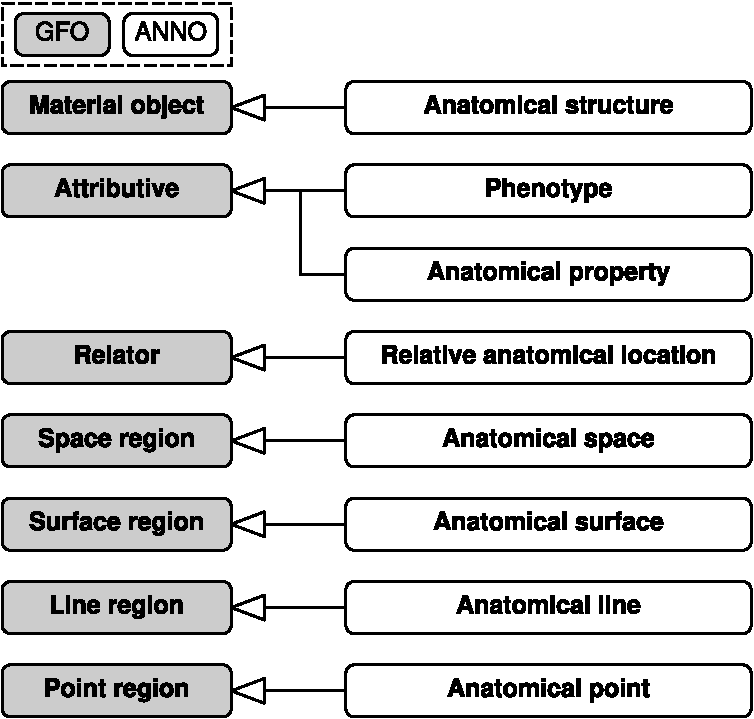
\includegraphics[width=0.6\textwidth]{img/gfo.pdf}
\caption{Integration of ANNO with the top-level GFO ontology.}\label{fig:gfo}
\end{figure}

%\section{Methodology for developing ANNO}
For the development of ANNO, we applied the onto-axiomatic method, a combination of the axiomatic method with a top-level ontology \citep{baumann2014, herre2010}.
The axiomatic method comprises principles for developing theories or formal knowledge bases, which aim at the foundation, systematisation and formalisation of a knowledge domain \citep{baumann2014, herre2010}.
When knowledge is systematized, a set of categories is considered \emph{primitive} or \emph{basic}.
Such categories are not explicitly defined, but implicitly described by axioms \citep{Hilbert1918}.
An example of a primitive category is \enquote{part}.
New notions can be introduced by explicit definitions based on the primitive or already defined categories \citep{herre2010}.

The considered axioms differ in their degree of abstraction.
At the most general level of abstraction, they are provided by top-level ontologies, whose axioms and categories can be applied to most domains of the world.
The onto-axiomatic method combines the axiomatic method with a top-level ontology, which is used to create more specialised core and domain-specific ontologies \citep{baumann2014}.
Possible ways of discovering axioms in empirical domains are generalisation based on single cases and idealisation \citep{baumann2011}.

We built ANNO on the basis of an ontology development schema that includes three main steps: 1. Domain Specification, 2. Conceptualisation and 3. Axiomatization \citep{herre2010}, and used the General Formal Ontology (GFO) \citep{Loebe2022, Burek2020, herre2010} as a top-level ontology in the sense of the onto-axiomatic method.

\paragraph{Domain specification}
As part of the domain specification, the anthropology experts conducted an extensive review of existing literature and ontologies, analysing and classifying the relevant information.
Together with ontologists, relevant use cases and competence questions\footnotemark{} \citep{XD2016, MOMo2023}, as well as views and classification principles of the objects in the anthropology domain \citep{herre2010} were discussed.
\footnotetext{queries that the ontology must be able to answer}
%
The following main use cases and competence questions (sub-items, selected examples) were defined:
\begin{enumerate}
\item Annotation of anthropological models (representations of anatomical entities) using a controlled vocabulary
\begin{enumerate}
\item Query all bone types
\item Query all parts (types) of a specific bone (type)
\item Query all parts (types) of a specific bone compound (type)
\item Query all tooth types
\item Query all parts (types) of a specific tooth (type)
\end{enumerate}
\item Specification of spatial relations between anatomical entities
\begin{enumerate}
\item Query all defined spatial relations
\item What is the relative anatomical location of an anatomical entity in relation to another anatomical entity?
\item On which anatomical structure does a defined measurement point lie?
\item Between which measurement points does a defined anatomical line lie?
\end{enumerate}
\item Specification of phenotyping functions
\begin{enumerate}
\item Query all phenotype specifications
\item Query the phenotyping function for determining a particular phenotype
\item Which parameters/variables (e.g., measurement distances/angles/points) are required to determine a particular phenotype?
\end{enumerate}
\end{enumerate}
Relevant domain objects were identified on the basis of the defined use cases.
These include bones, teeth, phenotypes, as well as spatial anatomical entities.
The objects are classified according to their type and part-whole relationship.

\paragraph{Conceptualisation}
During the conceptualisation phase \citep{herre2010}, the core concepts (categories, classes) and relations were introduced that form ANNOdc (domain-core ontology) (\cref{fig:annodc}).
The concepts were created by generalising and classifying the domain objects.
To answer the competence questions of the first use case, for example, a distinction must be made between whole bones, bone parts and composite bone structures.
Therefore, the corresponding concepts \enquote{Bone}, \enquote{Bone part} and \enquote{Bone compound} were introduced.
Further concepts were defined to represent spatial relations and phenotypes.
Furthermore, we identified relations (e.g., partOf, boundaryOf or locationOf) relevant to capture axioms covering the defined use cases, see \cref{fig:annodc}.

\paragraph{Axiomatization}
For the axiomatization and formal foundation of ANNO we utilised GFO as a top-level ontology and reused its categories, relations, axioms and modules (as a kind of Ontology Design Patterns \citep{ODP2005, XD2016, MOMo2023}).
We instantiated specifically the GFO modules \enquote{Material objects}, \enquote{Attributives} and \enquote{Space} \citep{Burek2020, Loebe2021, Loebe2018} and adapted them according to the requirements of the use cases.
Domain concepts introduced in the conceptualisation phase were embedded in GFO, i.e., defined as subcategories (subclasses) of certain GFO categories (fig. 1).
The required relations between the concepts were then either adopted from GFO or derived (specialised) from the corresponding GFO relation.
For example, GFO specifies that material objects occupy space regions \citep{Loebe2021}.
We integrated this pattern in ANNOdc by deriving the class \anno{AnatomicalStructure} from \aurl{gfo}{MaterialObject} and \anno{AnatomicalSpace} from \aurl{gfo}{SpaceRegion.}
In this way, we were able to adopt the whole axiom including the \enquote{occupies} relation between the two ANNO classes.
In a similar way, we applied the GFO pattern \enquote{point region is boundary of line region is boundary of surface region is boundary of space region} \citep{baumann2016} to the ANNO categories anatomical point, line, surface and space.
According to the GFO relator \citep{Loebe2018} pattern, we defined the class \anno{RelativeAnatomicalLocation} including the two roles: target (\anno{locationOf}) and reference (\anno{relativeTo}) anatomical entity. % (chapter $\ldots$).

Further axioms were introduced to precisely define certain categories.
In addition to an explicit textual definition of the category \enquote{Bone compound}, for example, we introduced the following axiom:
%
%\anno{BoneCompound}: \aurl{rdfs}{subClassOf} (\aurl{gfo}{hasPart} some (\anno{Bone} or \anno{BoneCompound} or \anno{BonePart}))
\begin{equation*}
\anno{BoneCompound} \sqsubseteq \exists \gfo{hasPart}.(\anno{Bone} \sqcup \anno{BoneCompound} \sqcup \anno{BonePart})
\end{equation*}
%
This axiom states that a bone compound consists of further bone compounds, individual bones or bone parts.
Another example axiom postulates that phenotypes can be derived from anatomical entities or anatomical properties:
%
%\anno{Phenotype}: \aurl{rdfs}{subClassOf} (\aurl{gfo}{derivedFrom} some (\anno{AnatomicalEntity} or \anno{AnatomicalProperty}))
\begin{equation*}
\anno{Phenotype} \sqsubseteq \exists \gfo{derivedFrom}.(\anno{AnatomicalEntity} \sqcup \anno{AnatomicalProperty})
\end{equation*}
%
Finally, a spreadsheet template was developed for domain experts to specify domain-specific entities (ANNOds), strictly compliant with ANNOdc, see \cref{sec:annodc}.
This means that the domain experts had to insert more specific categories (single categories or category trees) under defined ANNOdc core categories and to describe them by suitable annotations and relations introduced in ANNOdc.

The resulting OWL 2 ontology was generated using SMOG~\citep{smog} and validated by the HermiT~\citep{hermit} and Pellet~\citep{pellet} reasoners and SHACL shapes, see \cref{sec:annods}.
In both cases, the consistency of the ontology was proven.
As a use case, we integrated the ontology into the \aw{} software~\citep{aw3d} and were able to successfully realise all three intended use cases.
Thereby, most of the core categories,
such as \enquote{Bone}, \enquote{Bone part}, \enquote{Bone compound}, \enquote{Tooth}, \enquote{Tooth part}, \enquote{Phenotype}, \enquote{Relative anatomical location}, \enquote{Anatomical line} and \enquote{Anatomical point}),
and relation types (such as hasPart, boundaryOf, locationOf and derivedFrom) of ANNOdc were utilised and their subcategories and specific relations were dynamically queried (according to the three-ontology method).

The statistical information on the ANNO ontology is shown in \cref{tab:stats}.

\begin{table}[b]
\centering
\caption{Statistical information. Column values do not add up because some entities are defined in both subontologies.}
\label{tab:stats}
\begin{tabular}{lS[table-format=4.0]SSS[table-format=3.0]SS[table-format=5.0]S[table-format=3.0]S[table-format=3.0]l}
\toprule
% Expressivity according to Protege: ANNOdc and combined: ALCHIQ(D), ANNOds: ALE
Ontology	&\textnormal{Classes}	&\textnormal{Object prop.}	&\textnormal{Data p.}	&\textnormal{Individuals}	&\textnormal{Annotation p.}	&\textnormal{Axioms}	&\textnormal{FMA links}				&\textnormal{TA links} &Expressivity\\
\midrule
ANNOdc		&41						&11								&1								&0							&19				&178					&11							&0					&OWL DL\\
ANNOds		&1166					&0								&0								&803						&43				&18231					&503						&206				&OWL DL\\
\midrule
combined	&1195					&11								&1								&803						&53				&18382					&514						&206				&OWL DL\\
\bottomrule
\end{tabular}
\end{table}

\subsection{Description and foundation of ANNOdc}\label{sec:annodc}
The core ontology development occurs in close collaboration between ontologists and anthropologists.
The objective is twofold: to adequately represent the most basic anatomical and anthropological entities and to keep the ontology relatively simple and compact.
This approach ensures that domain experts can easily handle the ontology and efficiently integrate it into the \aw{} software, see \cref{sec:aw}.

% Definition/Beschreibung der Kern-Konzepte/Module und -Relationen mit Beispielen, GFO-Einbettung
\begin{figure}[h]
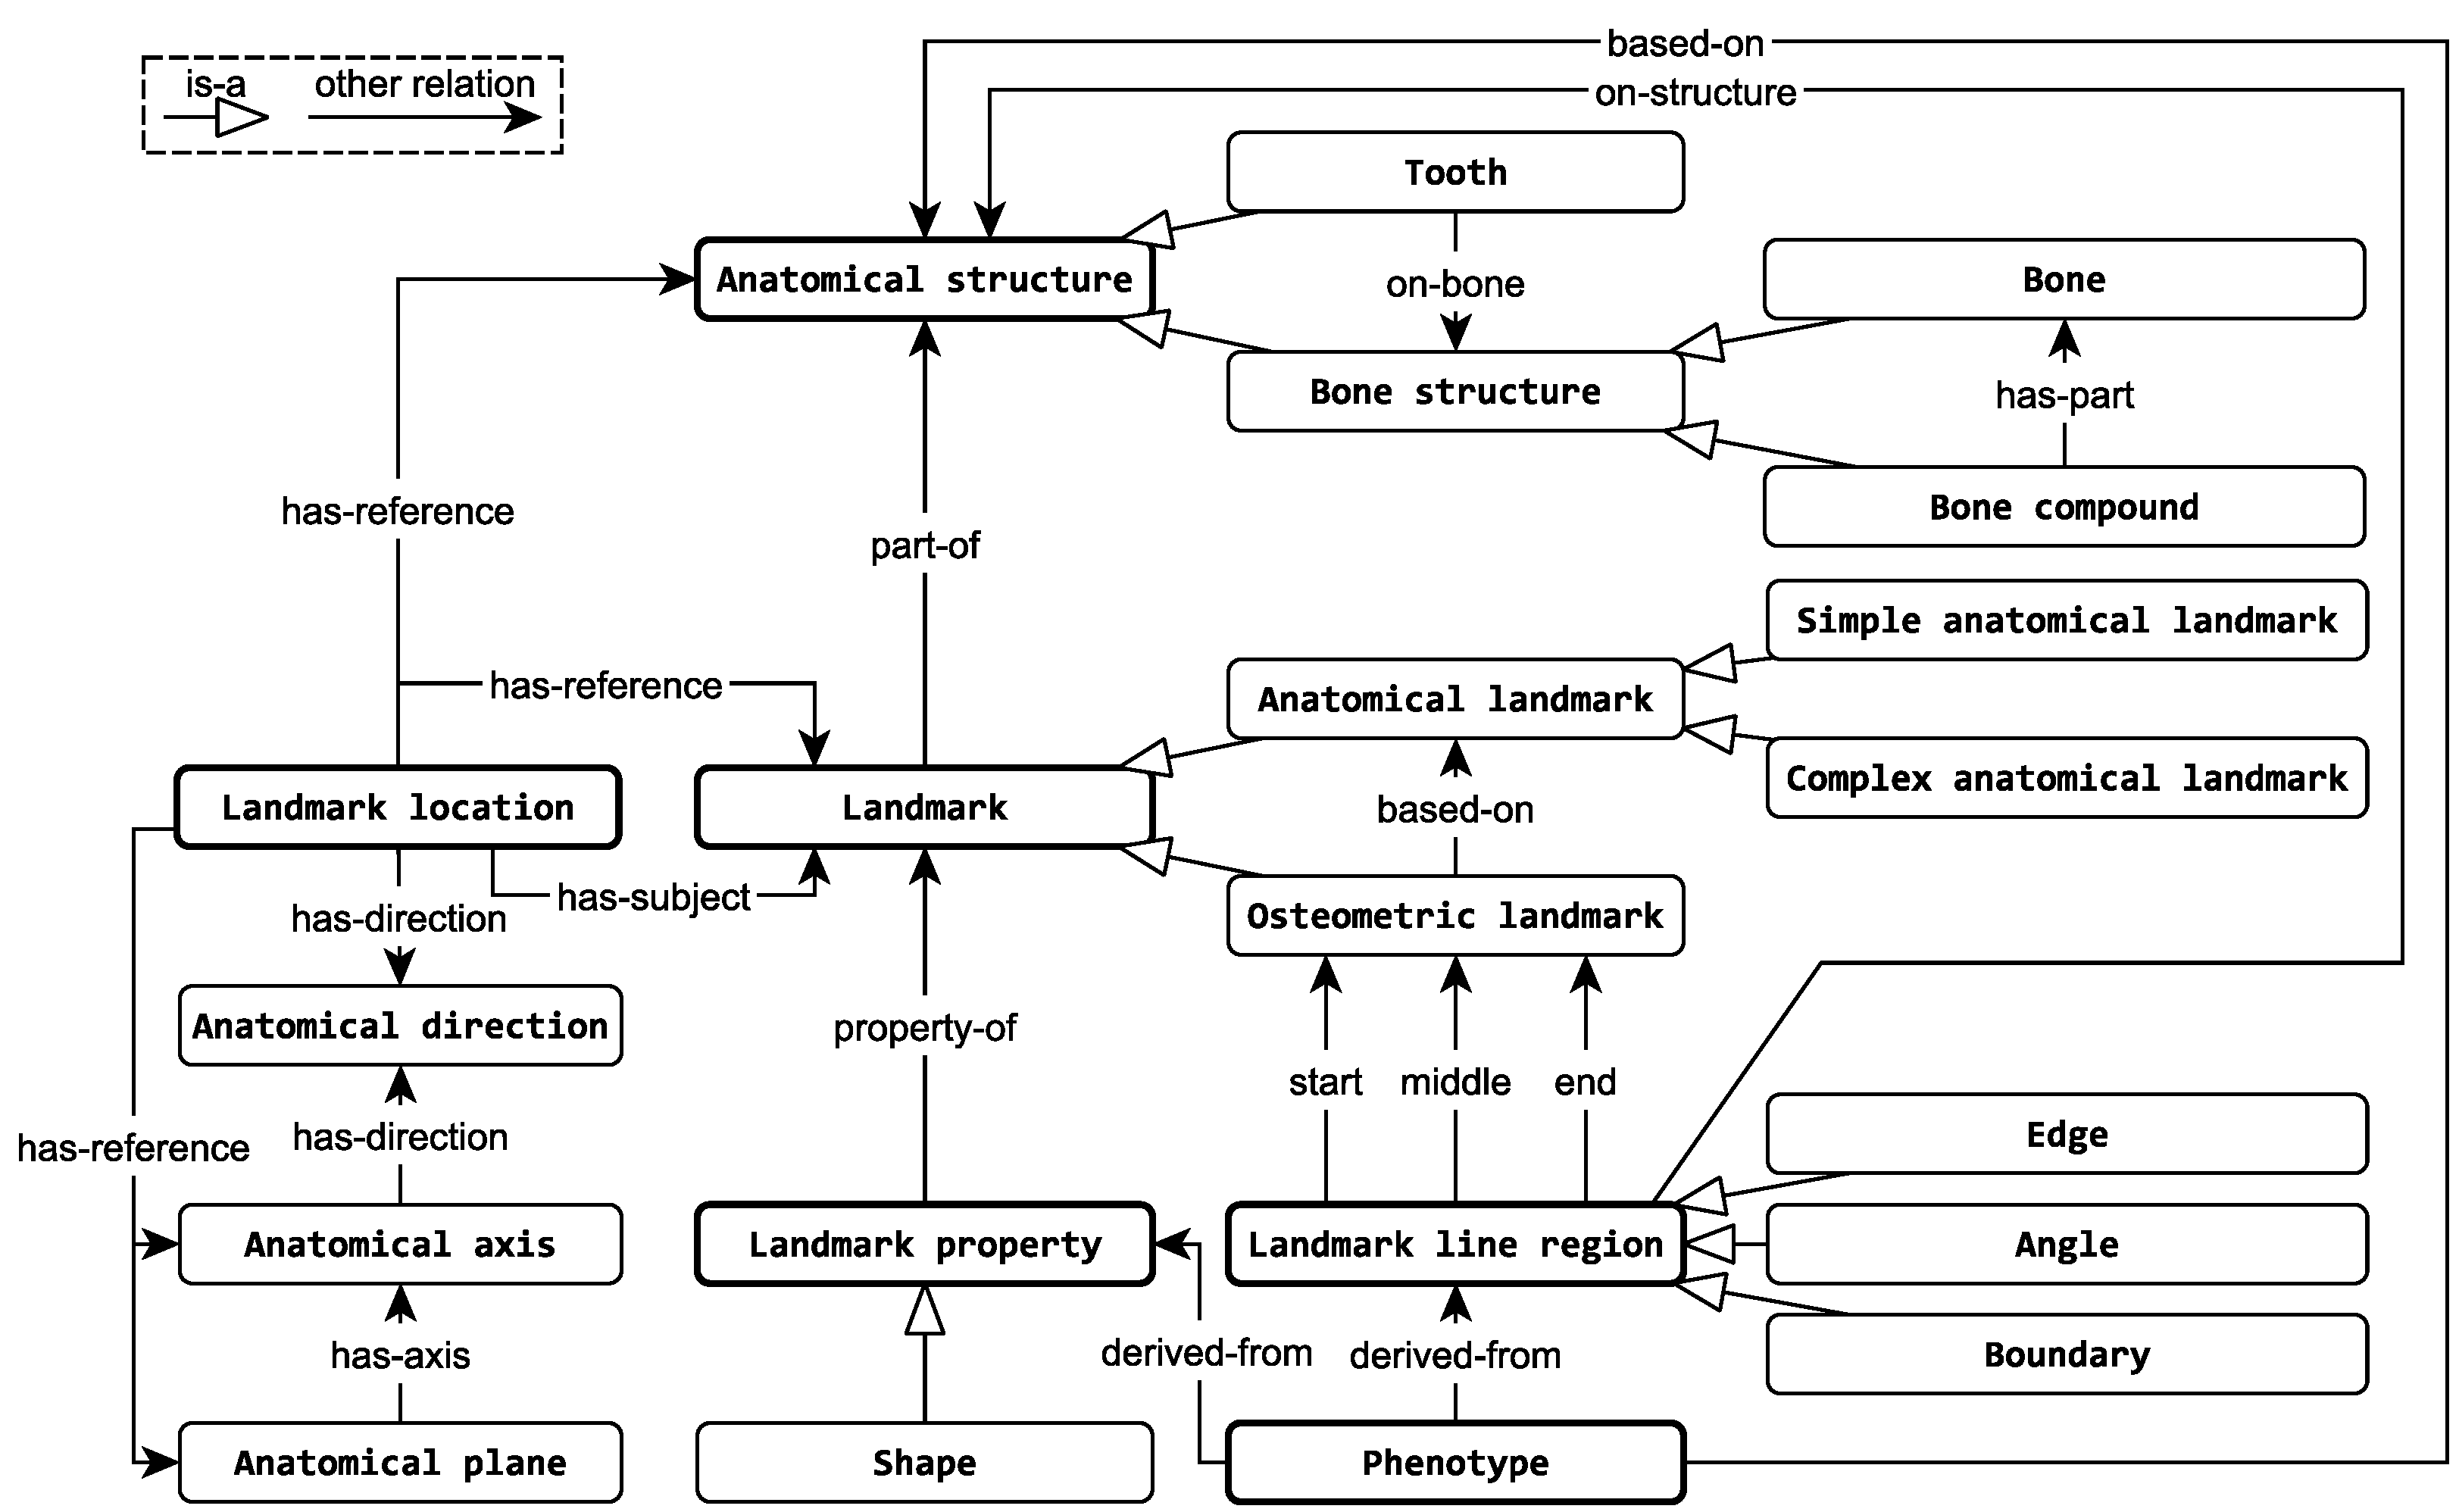
\includegraphics[width=\textwidth]{img/core.pdf}
\caption{The ANNOdc domain-core ontology.}\label{fig:annodc}
\end{figure}

\begin{table}[b]
  \centering
  \caption{Classes of ANNOdc along with exemplary ANNOds subclasses as well as interlinks to the FMA and the GFO top-level ontology.\\
  \textsuperscript{*} \anno{LO} is the line between \anno{Lambda} and \anno{Opisthion}, the \emph{occipital saggittal arc}.}
  \label{tab:core}
  \begin{tabulary}{\textwidth}{llLl}
    \toprule
	ANNOdc class					&ANNOds Examples				&FMA equivalent / ID						&GFO superclass	\\
	\midrule
	\anno{AnatomicalEntity}			&						&Physical anatomical entity \fma{61775}\\
	\anno{AnatomicalStructure}		&\anno{Skeleton}		&Material anatomical entity	\fma{67165}		&\gfo{MaterialObject}\\
	\anno{SpatialAnatomicalEntity}	&						&immaterial anatomical entity \fma{67112}	&\gfo{SpaceEntity}\\
	\anno{AnatomicalSpace}			&						&											&\gfo{SpaceRegion}\\
	\anno{AnatomicalSurface}		&						&Anatomical surface \fma{24137}			&\gfo{SurfaceRegion}\\
	\anno{AnatomicalLine}			&\anno{LO}\textsuperscript{*}	&Anatomical line \fma{9657}	&\gfo{LineRegion}\\
	\anno{AnatomicalPoint}			&						&Anatomical point \fma{9658}							&\gfo{PointRegion}\\
	\anno{MeasurementPoint}			&\anno{Lambda}\\%, \anno{Ophistion}\\
	\anno{OrientationPoint}			&\anno{Orbitale}\\
	\anno{AnatomicalPlane}			&\anno{FrontalPlane}	&Anatomical plane \fma{242982}\\
	\anno{AnatomicalAxis}		 	&\anno{SagittalAxis}\\
	%\anno{Skeleton}					&						&Osseous skeleton \fma{23875}\\
	\anno{BoneStructure}\\
	\anno{Bone}						&\anno{Mandibula}				&Bone organ \fma{5018}\\
	\anno{BonePart}					&\anno{ArcusAlveolaris}	&Related to Segment of bone organ \fma{281808}, Zone of bone organ \fma{10483}\\
	\anno{BoneCompound}				&\anno{Cranium}				&Comparable to union of Skeletal system \fma{23881} and subdivision of skeletal system \fma{85544}\\
	\anno{ToothStructure}\\%			&\anno{DentesPermanentes}\\%		&Permanent teeth (\fma{75152}\\%; TA2ID:913)\\
	\anno{Tooth}					&\anno{DensCaninus}			&Tooth \fma{12516}\\
	\anno{ToothPart}\\%\fma{56481}; TA2ID:925\\
	\anno{Phenotype}				&\anno{SexGiles19671}			&											&\gfo{Attributive}\\
	\anno{AnatomicalProperty}		&						&													&\gfo{Attributive}\\
	%\anno{AnatomicalProperty}		&Shape (Degree of morphological expression)	&Anatomical relation, e.g., Has\_shape &\gfo{Attributive}\\
	\anno{RelativeAnatomicalLocation}&\anno{Sinister}	&Anatomical qualitative coordinate \fma{30346}	&\gfo{Relator}\\
	%\anno{RelativeAnatomicalLocation}&superior, lateral, medial, posterior	&Anatomical qualitative coordinate	&\gfo{Relator}\\
\bottomrule
\end{tabulary}
\end{table}

%\paragraph{Terminology for descriptive anatomy}
\begin{figure}
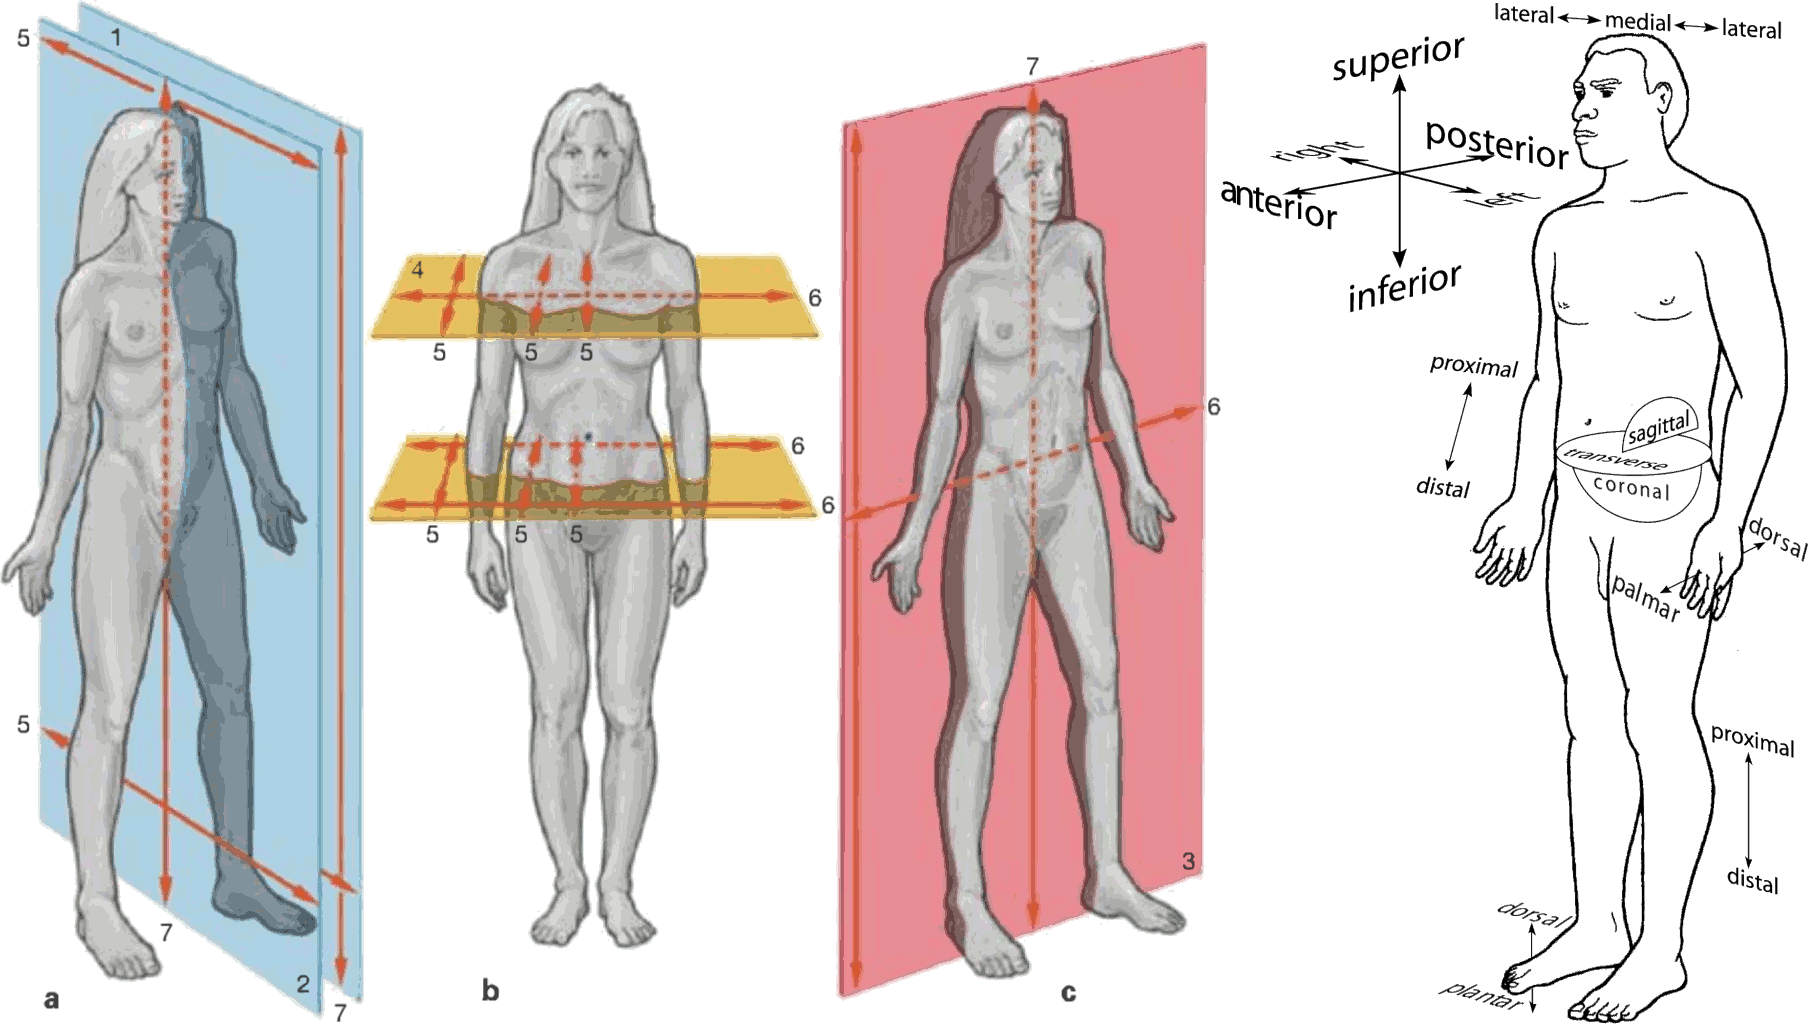
\includegraphics[width=\textwidth]{img/axisplanelocation.png}
\caption{Left: Anatomical Planes and Axes:
1 saggital plane,
2 midsaggital plane,
3 frontal plane,
4 transverse or horizontal plane,
5 saggital axis,
6 transverse axis,
7 longitudinal or vertical axis.
a: Planum sagittale (sagittal plane), includes sagittal and longitudinal axes; the midsagittal plane passes through the midline of the body,
b: Planum transversale (Transversal plane), includes transverse and sagittal axes,
c: Planum frontale (frontal plane): includes longitudinal and transverse axes.
Right: Anatomical relative location: directional terms used in anatomy and anthropology.
Modified figure based on \cite{allgemeineanatomieen,schemamann}.}
\label{fig:axisplane}
\end{figure}
%\FloatBarrier
The position of all anatomical entities is described in a standardized fashion using conceptual axes (a kind of anatomical line), planes (a kind of anatomical surface) as well as directions (relative anatomical locations).
Directions are relative to the body based on the standard anatomical position (\latin{Positio anatomica} \aurl{ta2}{72}, \aurl{fma}{23132}).
It refers to standing upright, facing forward, palms and toes pointing forward, thumbs to the side, and observed from the perspective of the respective individual. %Quelle kommt noch
%
Although an infinite number of axes and planes can be defined within the human body, generally three principal axes and planes are used~\citep{prometheus}.
They are mutually perpendicular and provide the three spatial coordinates.
The three principle axes, shown in \cref{fig:axisplane} are:
\begin{itemize}
\item The longitudinal or vertical axis runs in the superior-inferior direction in an upright position, perpendicular to the ground.
It intersects with the frontal and sagittal planes.
\item The sagittal axis runs in the ventral-dorsal direction, from the front to the back surface of the body and vice versa.
It intersects with the sagittal and transverse planes.
\item The transverse or horizontal axis extends from left to right, intersecting with the frontal and transverse planes.
\end{itemize}

The three principal planes, depicted in \cref{fig:axisplane}, are:
\begin{itemize}
\item The sagittal plane, i.e all vertical planes parallel to the sagittal suture of the skull and running from anterior to posterior in the upright position.
The median (sagittal) plane divides the body into two symmetrical halves.
\item The frontal plane (= coronal plane) comprising all planes parallel to the forehead (frons) or the coronal suture of the skull, running vertically from one side of the body to the other in the upright position.
\item The transverse plane including all horizontal cross-sectional planes, relative to the upright position, dividing the body into cranial and caudal sections.
They run perpendicular to the longitudinal axis of the body.
\end{itemize}

Each one has two anatomical axes as boundaries in the sense of GFO, which allows boundaries to occur inside a structure and not necessarily at the extremities.
For example, the coronal (frontal) plane has the transversal (horizontal) and longitudinal (vertical) axes as boundaries.

An anatomical direction or relative anatomical location, as shown in \cref{fig:axisplane}, is the position of an anatomical entity (e.g., a bone structure) in relation to another anatomical entity (e.g., another bone, an axis, a plane or a point such as the center of the body).
Relative anatomical locations are classified according to the anatomical terms of location (e.g., cranial or superior = \enquote{towards the end of the skull}, dexter = \enquote{right} or distal = \enquote{in direction towards the end of a limb}).
For example, the Glabella is located laterally to both Arcus superciliaris (Arcus superciliaris sinister and Arcus superciliaris dexter).
A relative anatomical location can be considered as an individual relation between two anatomical entities (target entity and reference entity) and can therefore be modeled using a GFO relator.
Relators are composed of roles (in our case target and reference) and have the power to relate arbitrary entities (in our case, anatomical entities)~\citep{gfocategory}.

%\paragraph{Anatomical entities}
An anatomical entity is either an anatomical (material) structure or a spatial anatomical entity, such as \anno{Cranium} or \anno{FrontalPlane}.
An anatomical structure refers to any anatomical division or material anatomical entity.
ANNO describes three kinds of anatomical structures: tooth structures (teeth and teeth parts), bone structures (single bones, bone parts and bone compounds), as well as the complete skeleton.
The GFO defines a material object \aurl{gfo}{MaterialObject} as a solid concrete entity that belongs to the material region of the world, has mass, consists of matter and occupies space~\citep{gfospace}.
Accordingly, we define \aurl{anno}{AnatomicalStructure} as a \aurl{gfo}{MaterialObject} in the anthropological context.
The closest equivalent in the FMA is the \emph{Material anatomical entity} \aurl{fma}{67165}, the subclass of \emph{Physical anatomical entity} \aurl{fma}{61775} that has mass.

%\paragraph{Skeleton}
The largest or most comprehensive skeletal anatomical structure, the human skeleton, is the framework composed of all the bones and teeth of a human being.
The TA~\citep{ta2} equates the skeleton with the \enquote{Systema skeletale (skeletal system)}, which refers to the passive part of the musculoskeletal system, including the articulated bony skeleton with teeth, as well as cartilage, ligaments, and other joints.
ANNO does not adopt this equivalence, and \enquote{Skeleton} here refers to the entirety of a human's bones and teeth.
However, since teeth constitute their own tissue, they are treated separately, allowing all other components of the skeletal system, such as cartilage or ligaments (as tissues) or joints (e.g. as specific aspects), to be integrated and referenced separately in ANNO.
The anthropologically meaningful distinction between \enquote{Skeleton} and \enquote{Systema skeletale} can be maintained, while still referencing both within the TA concept.

%\paragraph{Tooth structure}
Tooth structures comprise teeth and their parts.
A human tooth is an individual unit of the human dentition (synonymous for the teeth as a whole).
Teeth are part of the skeleton, yet they are characterized by their own distinctive tissue and thus treated separately from bones.
Teeth, such as the Dens caninus (canine tooth) are located on bone structures.
The FMA has the equivalent class \enquote{Tooth} \aurl{fma}{12516}.
A tooth part is any portion of a tooth.
They are not included in the initial scope of the ontology, but they are one of the aspects by which it can be expanded.

%\paragraph{Bone structure}
Bone structures comprise all possible parts of the human skeleton, which are individual bones, bone parts, bone compounds as well as the complete skeleton excluding the teeth.
The FMA does not have a common superclass for those parts but instead mounts them in different parts of its hierarchy.

A bone or bone element is a single self-contained bony skeletal entity.
Bones, such as Mandibula (Mandible) and Os occipitale (Occipital Bone) are individual bone organs.
FMA does have a \enquote{Bone} class (\aurl{fma}{30317}) but that only has a single subclass \enquote{Skull bone} (\aurl{fma}{30317}).
Instead, \enquote{Bone organ} (\aurl{fma}{5018}) is the equivalent class.

A bone compound is a section of the skeleton combining multiple bones or bone parts together, depending on the classification system chosen.
This allows for the representation of any partonomy that need not necessarily be compatible with one another.
Bone compounds, such as the Cranium (skull bone) consist of further bone compounds, individual bones (which in turn consist of bone parts) and bone parts.
The FMA does not have a single equivalent class, but it is similar to the union of \enquote{Skeletal system} (\aurl{fma}{23881}) and \enquote{Subdivision of skeletal system} (\aurl{fma}{85544}).
On the skeletal level, bone parts comprise any piece or portion of a bone.
An anatomical landmark is any distinct structure on a bone.
In ANNO, it is also referred to as a bone part.

%\paragraph{Spatial anatomical entity}
An anatomical entity without mass is classified as a spatial anatomical entity, which is either an anatomical space (three-dimensional), an anatomical surface (two-dimensional), an anatomical line (one-dimensional) or an anatomical point (zero-dimensional).
It is equivalent to the FMA \enquote{Immaterial anatomical entity} (\aurl{fma}{67112}).

An anatomical space is a space region (three-dimensional) occupied by an anatomical structure.
An anatomical surface is a boundary (two-dimensional) of an anatomical space.

An anatomical point (or osteometric landmark) is any immaterial, conceptual point that marks a location on a bone, either to create measurements (anatomical lines) or locate other anatomical points, e.g. by aligning the bone in specific planes for a measurement.
The former serve as measurement points, the latter - relevant to the measurement procedure as orientation points.
An anatomical point is thus a boundary (zero-dimensional) of an anatomical line.

An anatomical line is a conceptual, immaterial line on a bone passing between at least two measurement points that, in the form of distances, circumferences or angles is used to collect measurements representing aspects of a bone's dimensions.
An anatomical line is a boundary (one-dimensional) of an anatomical surface.
Anatomical lines can connect or pass through anatomical entities (e.g., an edge between two or an angle between three anatomical entities).
The length of the line or the angle degree can be measured and used in functions to infer individual phenotypes.% [Verweis zu Phenotype section].
For example, the anatomical line \anno{ZyDexterumZySinistrum} between the \latin{Zygion Dexterum} and the \latin{Zygion Sinistrum} is used in the sex determination function for the phenotype \anno{SexGilesElliot196319}~\citep{sexgileselliot1963}.

%\paragraph{Phenotypes and anatomical properties}
\begin{figure}[h]
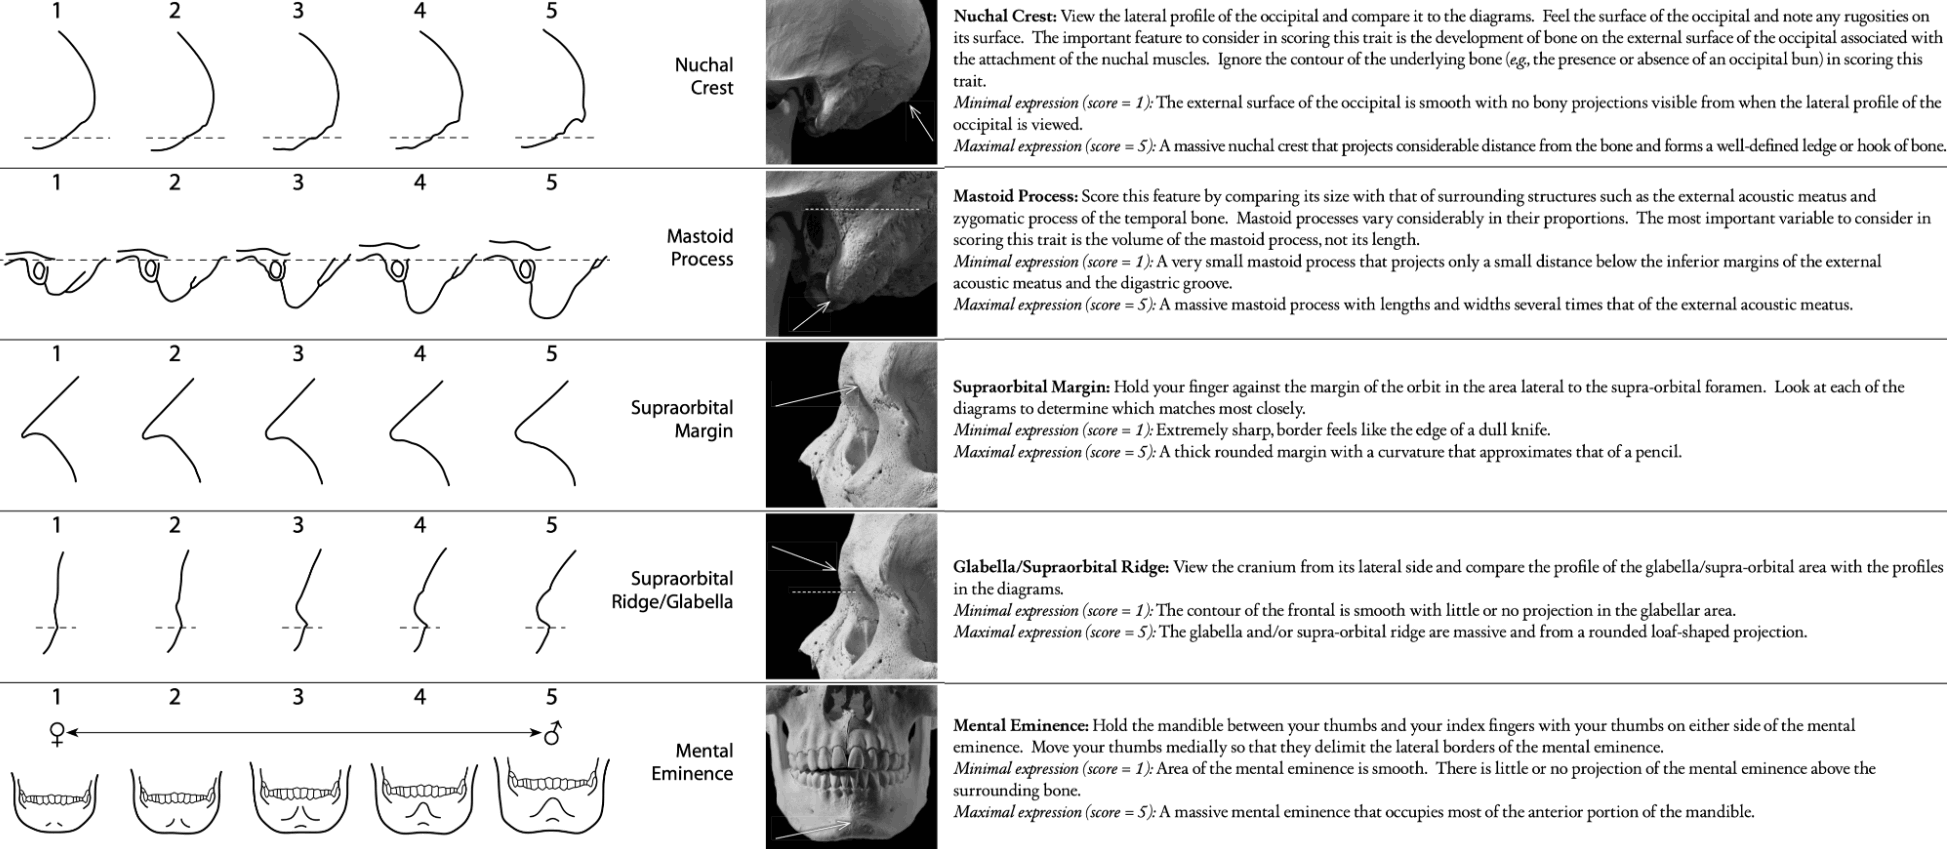
\includegraphics[width=\textwidth]{img/phenotype.png}
\caption{
Exemplary assessment of anatomical properties for the derivation of the phenotype sex, where five cranial bone parts are evaluated for their level of morphological expression.
% yes, walker method is published in buikstra
Method after Walker~\cite{datacollection}.
Image taken unmodified from \cite{datacollection}.
}\label{fig:phenotype}
\end{figure}

Usually, a phenotype is considered as a (combination of) bodily feature(s) or observable characteristic(s) of an organism, such as sex, body height or body weight~\citep{ontologicaltreatment,phenomes,interoperability}.
Since phenotypes are individual properties, they can be considered as attributives in the GFO sense.
The phenotype notion has also been analyzed in detail within the framework of the Core Ontology of Phenotypes~\citep{ontologicalrepresentation}.

In the case of ANNO, the phenotype can be derived using functions comprising obtained measurements.
Discriminant functions, e.g. based on the Cranium, allow for the assignment to sex while estimation of stature is attained by using linear regressions, e.g. based on Femur or Tibia length measurements.
RDF is not optimized for mathematical formulas so we model those as literals.

% ć in Vodanović cannot be displayed without font package and I don't know if the journal allows a different font
As an example, the discriminant function no. 6 developed by Vodanovic uses the measurement of the angus mandibulae to assign sex, thus deriving a phenotype.
For the left side it is given as:
\[
0.17 \cdot [\text{ppam sinistrum-go sinistrum-paim sinistrum}] - 20.43
\]
The right side is calculated analogously using (ppam dexterum-go dexterum-paim dexterum).
%\[
%\text{For the right side: } ([\text{ppam dexterum-go dexterum-paim dexterum}] \times 0.17) - 20.43
%\]
The threshold or sectioning point is given at 0.2, meaning that if the result is greater than this value, then sex is assigned to male, if it is lower it is assigned to female.

%\paragraph{Anatomical property}
An anatomical property is a characteristic (e.g., shape) of an anatomical structure.
Anatomical properties are considered as attributes or qualities in GFO~\citep{gfoarchitecture}.
These are dependent individuals that characterise other individuals (in our case, anatomical structures).

Other than by means of osteometry using measurements and functions, an anatomical landmark's morphology can be used to examine anthropological aspects or phenotypes such as age or sex.
For instance, assessment of the degree of an anatomical landmark's morphological expression (the anatomical property in this case) offers information about the sex of the remains of the individual being examined.
While the morphological examination was not within the scope of the project, it was nonetheless ensured that future extension in this respect is possible.

\subsection{Development of ANNOds}\label{sec:annods}
While ANNOdc is created by the ontologists in consultation with the domain experts, ANNOds is developed by the domain experts themselves.
%The primary focus is on the design of ANNO's ontological architecture and the conception of the process for creating the content, as well as on the integration into the Applied University of Mittweida's in-house software \aw{}.
For this purpose they were provided with a spreadsheet-based SMOG~\citep{smog} template by the ontologists, see \cref{fig:smog}, eliminating the requirement of having a background in RDF and ontologies.
The template is based on the structure of ANNOdc, so that the entered data is compliant with it: The ANNOds classes are subclasses of the ANNOdc classes (see \cref{tab:core}) and properties (see \cref{fig:annodc}) from ANNOdc are used.
The spreadsheet is transformed to an OWL 2 ontology consisting of a taxonomy, annotations and some simple axioms on the basis of property restrictions.
This approach ensures intuitive and unimpeded data input and a valid end result.
Additionally, ANNOds is validated using SHACL shapes\footnote{Contained in \texttt{dist/shacl.ttl} in \url{https://zenodo.org/record/8380382}.}, which requires metaclasses.
For example, all directly specified and transitive subclasses of \anno{Bone} are also explicitly individuals of the metaclass \anno{BoneClass} because of the limitations of SHACL.
In addition, the objective is to initiate the process of data entry, encompassing selected bones of the skeleton.

\begin{figure}[ht]
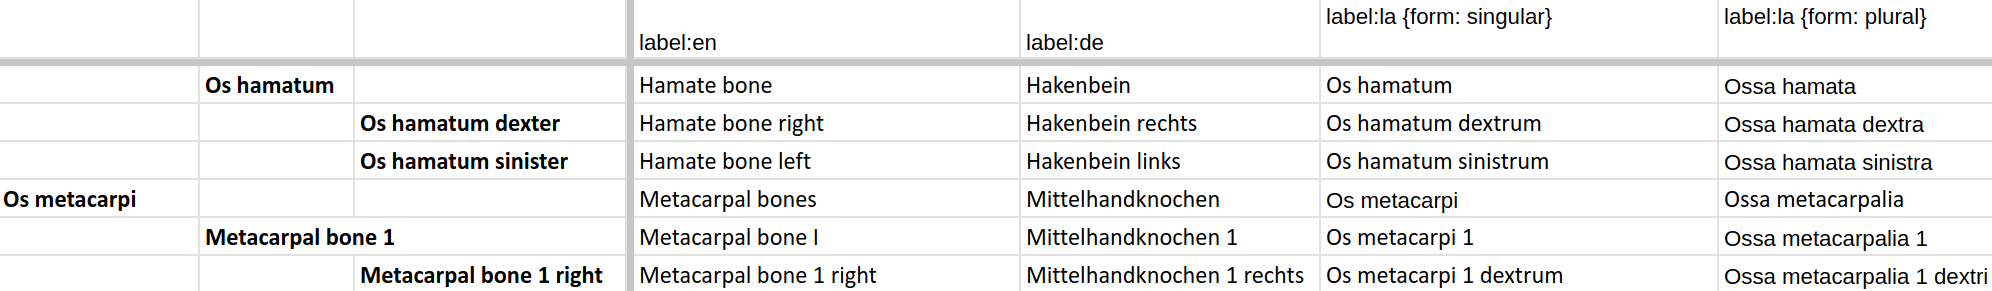
\includegraphics[width=\textwidth]{img/smog.png}
\caption{Excerpt of the spreadsheet-based input template used by the anthropologists.}\label{fig:smog}
\end{figure}

%\subsections{General considerations}
ANNO thoroughly delineates each concept with precise terminology, definitions, and clear distinctions for identifying features or taking measurements, with all information backed up by detailed source citations for transparency.
All bone structures and anatomical points are annotated with their name in singular and plural form, reference bone, synonyms, textual and visual definition, FMA and TA ID, and sources.
%
%Anatomical Landmarks (Bone Parts) (Selection Criteria, scope and process, properties)
%Osteometric Landmarks (Anatomical Points)
%Measurements (Anatomical line)
Measurements for determining phenotypes involve relevant spatial anatomical objects (e.g., lines), which are defined by the anatomical points or objects that delimit them.
These include references to specific sections, the starting point, midpoint, and end point, accompanied by concise definitions.
%Phenotypes
%Development of the ontology is based on the following selection criteria:
%The selection criteria are as follows:
Given the overwhelming number of bone parts present in the cranium, the initial selection was narrowed down to a selection of representative and relevant parts.
Overall, however, the aim is to include those that are of anthropological relevance, i.e. that contribute to navigation, localization, and identification on the bone.
Those structures included in the definitions of others were also to be defined.
For bones that lie on the median sagittal plane (e.g., mandible or sternum), bilateral landmarks are defined, each with a side reference.
For osteometric landmarks, all those already established in the core literature are to be used.
Furthermore, those that are relevant for meaningful measurement distances and can be annotated in \aw{} should be used.
For the measurement distances, those should be selected that are established in the majority of the core literature as well as necessary for discriminant functions and functions for estimating height and weight.
%In addition, it also had to be integrable into \aw{}.
The functions chosen were those with diagnostic value.
These were discriminant functions for sex determination and regression functions for body height and body weight estimation.

%\paragraph{Process for creating definitions and measurements}
For the definitions and measurements, a representative minimum amount of anthropological and anatomical English- and mostly German-language literature was compared in order to develop the definitions from their information.
Notably, Latin or latinized ancient Greek terms often missing in the English literature and the FMA were included.
%The FMA also contains only English terms.
%For this reason, these were also searched with their synonyms.
Overall, the name of the structure, measurement or point is noted in Latin in singular and plural forms, English, German, synonyms in all three languages, the FMA and TA ID, and any information on function and delineation.
This requires a positional description, such as the Punctum superioris capitis femoris as the superior located point of the Caput femoris.
%The examination of the Latin grammar was relevant for this.
For the measurements, in addition to the name of the measurement, the type (e.g., distance measurement) and the measurement instrument were also recorded.
The subsequent visual definitions were made in the different anatomical views marking the area of the anatomical structures and the position of the anatomical points.

%\paragraph{Functions}
The functions are divided into discriminant functions for sex determination and regress functions for body height.
The sex of a specific individual within a population may be estimated using a function on skeletal measurements that is specific or similar to this population.
Based on a threshold value, skeletons are classified into male, probably male, indifferent, probably female, and female.
The exact number of categories may vary depending on the particular method used.
ANNOds covers functions for at least one European, African, American, and Asian ethnicity or population.
%Names are assigned by the number included in each study, the authors, and the year of publication.
%In addition, the function, reference population, aspect (e.g., discriminant function), and sample size with division by gender are noted.
%For the discriminant functions, the thresholds of sex assignment, classification accuracy, and misclassification are important; for the regression functions, the error interval is important.
%
%While there are many textual sources of anthropological systematisation, they do not agree in all aspects and there is not a single, formally described, standard.
%ANNO links to concepts of the FMA when they exist, but structures them in a different way.
%
%\paragraph{Sex determination}
% auto translated from the project report, use as basis:
%
%\paragraph{Regress functions}
%Regress functions for body height and body weight estimation.
%Names were assigned by the number included in each study, the authors, and the year of publication.
%In addition, the function, reference population, aspect (e.g., discriminant function), and sample size with division by gender were noted.
%In addition, for the discriminant functions, the thresholds of sex assignment, classification accuracy, and misclassification were important; for the regression functions, the error interval was important.
%
%Standardised description of position
%In addition to the conception and development of the ontology as well as of definition, data input was initiated as content of Cranium including the Mandibula as well as the teeth of the was entered.
%Entries can be added directly to the OWL-File using Protégé or they can continue to be entered directly into the spreadsheet.
%In the latter case, the OWL file can be generated with a custom OWL generator.

%\paragraph{Validation}
%When transforming the input sheet to ANNOds, SMOG~\citep{smog} executes some basic validation heuristics, such as warning on undefined references.
% pyshacl mit metaklassen wäre möglich

\paragraph{Resolving incongruities}
\begin{figure}[h]
\centering
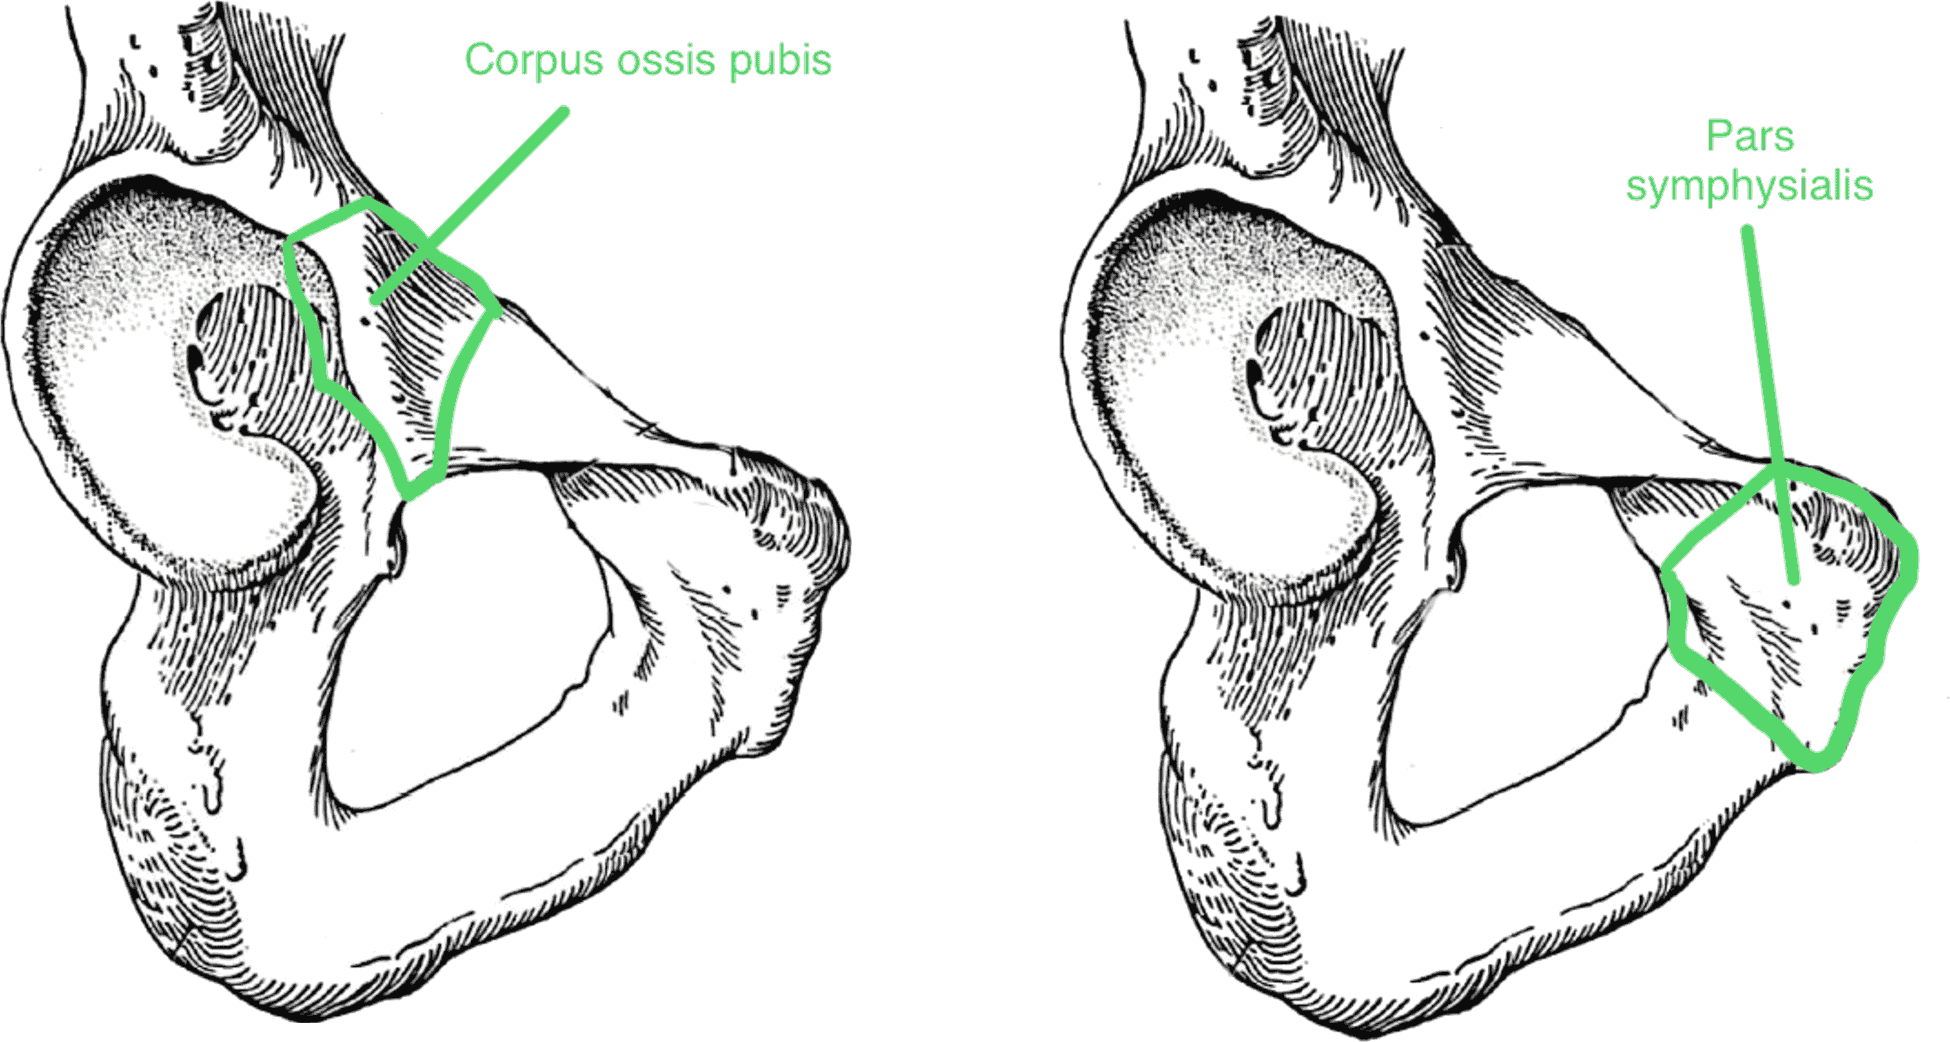
\includegraphics[width=0.6\textwidth]{img/corpus_ossis_pubis.png}
\caption{The \latin{Corpus ossis pubis} (pubic body) forms the proximal part of the \latin{Os pubis} and includes the anterior part of the \latin{Acetabulum} as well as the \latin{Eminentia iliopubica}, which is a small elevation on the \latin{Corpus ossis pubis}.
According to the \emph{TA} and others~\citep{ta2,schemamann,anatomylexicon2007,drake2019gray,anatomylexicon,prometheus2,anatomie}, this landmark is located in the region of the \latin{Facies symphysialis}, which is defined here as the \latin{Pars symphysialis}.
}\label{fig:corpusossispubis}
\end{figure}

The domain experts reconciled conflicting literature to arrive at a consistent and logical result, for example for the \latin{Corpus ossis pubis}, see \cref{fig:corpusossispubis}:
Since the Corpi of the \latin{Os ischii} and \latin{Os ilii} are located in the area of the \latin{Acetabulum},
it is logical to place the \latin{Corpus ossis pubis} in this region as well~\citep{graysanatomy,waldeyer,allgemeineanatomie,datacollection2,romanianmandible}, thereby forming the \latin{Acetabulum} from all Corpi (\latin{Corpus ossis ilii}, \latin{Corpus ossis ischii}, and \latin{Corpus ossis pubis}).
The \latin{Pars symphysialis ossis pubis} has ventral-medially the \latin{Facies symphysialis}, which connects the paired \latin{Ossa pubes} of the pelvic bones.
In the \latin{Pars symphysialis}, the \latin{Ramus inferior ossis pubis} and \latin{Ramus superior ossis pubis} merge into each other.
This redefinition closes the resulting gap in the definition of the area between the Ramus \emph{inferior / superior} ossis pubis.
%
ANNO also corrects the commonly missing differentiation between \emph{Cranium} and \emph{Mandibula} in English literature, with no Latin equivalent for the overall term \enquote{skull}.
Instead, \anno{Cranium} is established as a synonym for the skull~\citep{allgemeineanatomieen,prometheus2}.
\paragraph{}

Further contributions of ANNO include ensuring consistent Latin declension, including the plural form; enhancing transparency with detailed source references, distinguishing between original (primary) and citing (core) sources in the case of measurements.
The ontology dissects group structures into atomic bone parts and more moreover introduces new terms and definitions for landmarks such as joint surfaces, which, despite their anthropological relevance, often remain unnamed in anatomy literature.
It also formally establishes terms for osteometric measurement points outside the skull, addressing gaps not covered in the existing literature.

\section{Use Case: Integration into \aw{}}\label{sec:aw}
%\section{Use Case: Integration into \aw{}}\label{sec:aw}

\aw{}, see \cref{fig:aw}, is a German-language tool that combines user-friendly techniques of photogrammetry with insights from user experience research and knowledge from game development.
It enables users to virtually examine digitized bone material, which can be created using a procedure designed for generating 3D models of bones.
These models serve as digital twins in anthropological, morphological, and osteometric research and examination.
To facilitate such examinations, the software can import and render these 3D models at runtime and provides a comprehensive suite of tools for annotating and measuring bone material.
This facilitates anthropological work to be location-independent and parallel without exercising wear and tear on the skeletal material.
The examination can be performed as often as desired, even if the skeletal individuals or collections are not available at the institute or have already been reburied.

The ANNO ontology was created to be used in conjunction with \aw{} and was integrated into the software to better meet the use cases of the program.
These use cases include the annotation of bone material through markings in 3D space on the bone models, including point, line, and surface markings.
They also involve the measuring of bones by providing line, circumference, and angle measurement tools for use in osteometrical contexts.
To improve the quality of the annotations and measurements additional information such as alternative titles and descriptions, and others can be input by text.
Moreover, the software offers the capability to display either the entire skeleton or specific parts, thereby enhancing the examination context.
This feature enables users to not only focus on the specific bone they are studying but also easily access adjacent or related bones for a more comprehensive understanding.
These use cases are already covered by \aw{} itself but are improved by an integration of ANNO into the software.
Additional use cases that are only achievable through this integration include the automatic derivation of bone and skeletal phenotypes using mathematical functions available in the ontology and the provision of anthropological, anatomical and osteometrical knowledge for users through ANNO.

\begin{figure}[h]
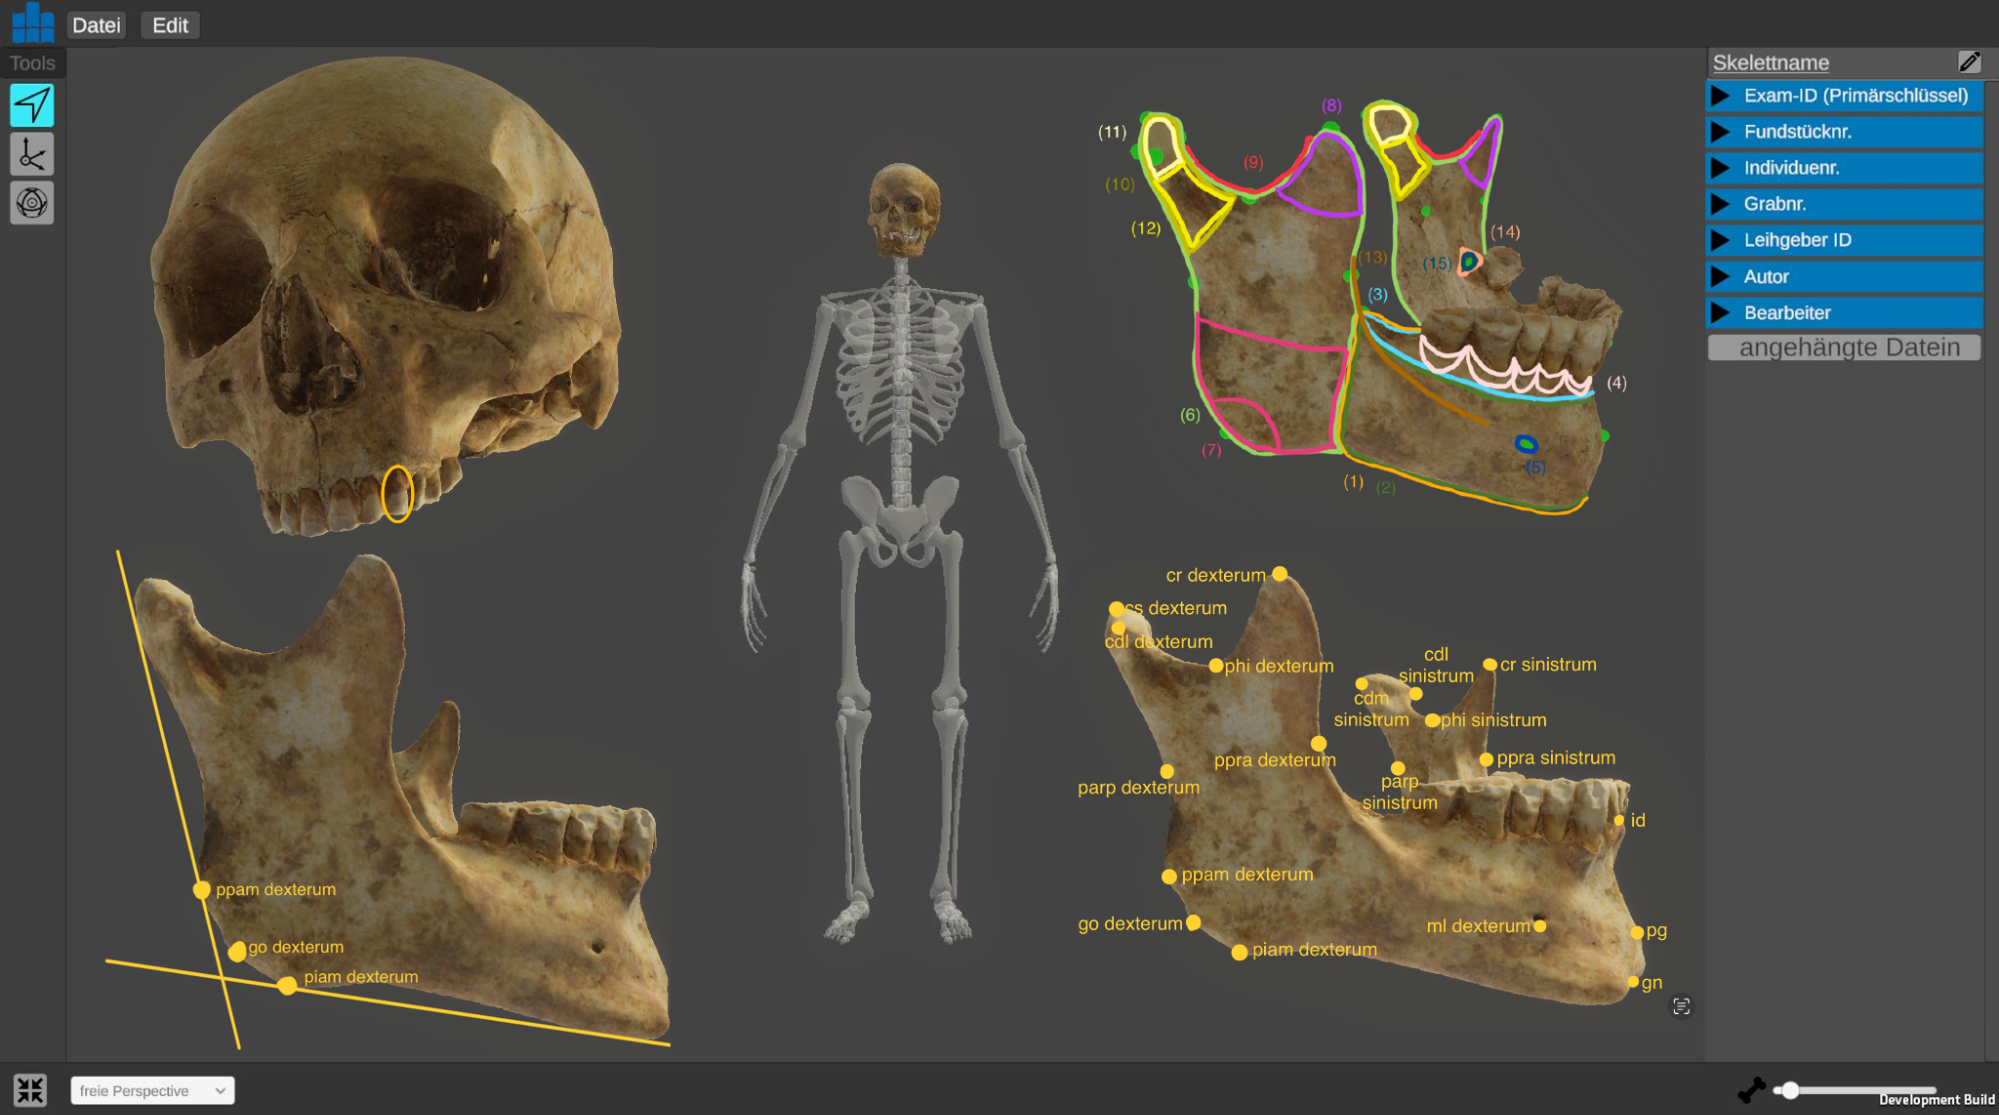
\includegraphics[width=\textwidth]{img/aw3d.png}
%\caption{3D model of a Cranium (skull) inserted into a placeholder skeleton in \aw{} depicting examples of various ANNOdc classes.}
\caption{
Collage of different views in \aw{} of a 3D model of a \emph{cranium} (skull) inserted into a placeholder skeleton (source:~\cite{aw3dcidoc}).
The cranium is a bone compound consisting of 29 bone elements.
One of them, the \emph{mandibula} (mandible), is flexibly connected to the rest of the skull by the mandibular joint.
In the top right, various bone parts on the Mandibula are visually emphasized, with part 7 representing the angulus mandibulae (mandibular angle).
In the top left, the \latin{Dens caninus maxillaris dexter} (right maxillary secondary canine tooth), a tooth structure, is highlighted within a circle.
The tooth cusp is a part of the tooth.
It refers to the projection that divides the occlusal surface of most of the teeth, with the exception of the incisors.
At the bottom right, anatomical points (osteometric landmarks) of the right lateral side of the \emph{mandibula} are depicted.
The \latin{Gonion dextrum} (right gonion, abbreviated as \latin{Go dextrum}, depicted alternative spelling of dextrum: dexterum) forms part of an anatomical line measuring the \latin{Angulus mandibulae},
as shown in the bottom left.
Skeletal material courtesy of Dr. Birgit Grosskopf, Department of Historical Anthropology and Human Ecology, University of Göttingen.
}
\label{fig:aw}
\end{figure}

We use our ontological architecture (top-level ontology, domain core ontology, domain specific ontology) to integrate ANNO into \aw{} based on the three-ontology method~\cite{threeontologymethod}.

\begin{figure}[h]
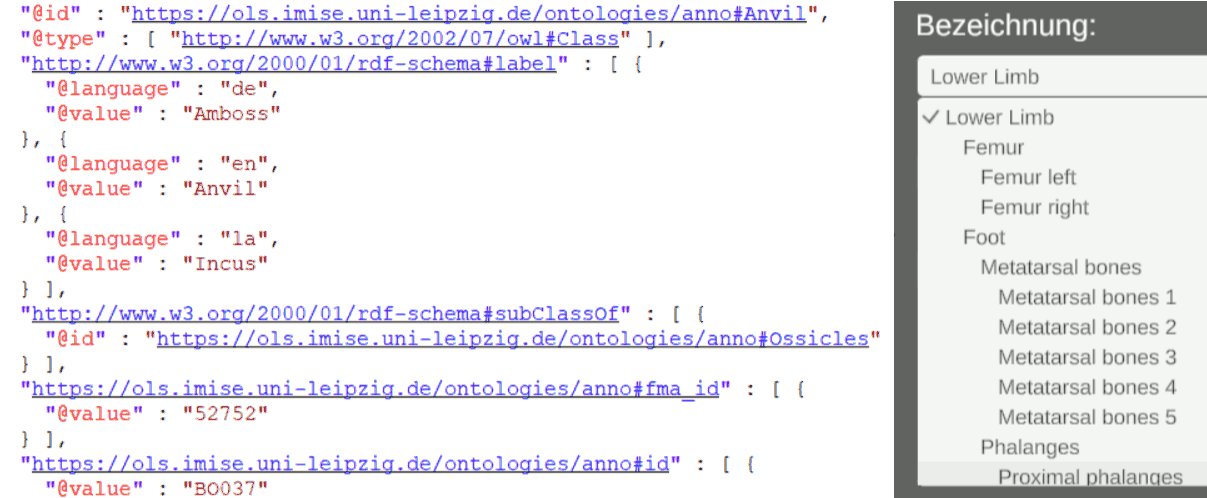
\includegraphics[width=0.7\textwidth]{img/json.png}
\caption{Left: ANNO converted to the \aw{} JSON input format. Right: Bone selection in the imported hierarchy.}
\label{fig:json}
\end{figure}

%This method, as outlined in~\cite{threeontologymethod}, aided us in designing a tool for annotating human skeletons and identifying phenotypes.
%We use ANNOdc as the Task Ontology and ANNOds as the Domain Ontology.
One of the advantages of the three-ontology method is that the software only needs to implement access to the entities (classes and properties) of ANNOdc ontology, whereas the classes of ANNOds are processed dynamically, as shown in \cref{fig:json}.
%\aw{} leverages ANNOdc as an interface to dynamically access the entities of the ANNOds, such as listing all subclasses of a specific class like \aurl{anno}{Bone}, as explained in \cref{sec:aw}.
%
In addition, it is now possible to perform sex determinations using discriminant functions, as shown in \cref{fig:function}.

\begin{figure}[h]
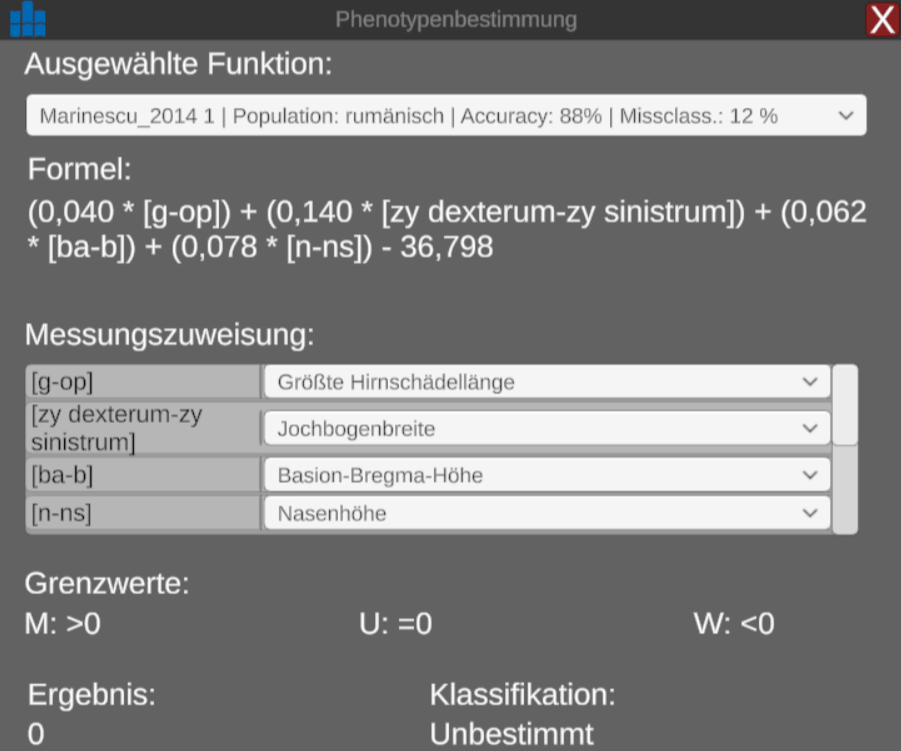
\includegraphics[width=0.4\textwidth]{img/function.png}
\caption{Sex determination in \aw{} using the imported ANNO discriminant functions.}
\label{fig:function}
\end{figure}

%%%%% the following part is removed
\iffalse
It also draws its advantage when space is limited.
Thus, it requires only three SLR cameras, sufficient exposure and a computer.
The examination proceeds as follows: After photogrammetry is done and the 3D model is created, the objects are imported into the software and calibrated.
For calibration, there is an individual placeholder for each bone, which must first be selected.
Then the calibrated digital twin is placed in a placeholder skeleton.
Annotations can be made in the detailed view of each bone.
Point, line and area markings are available for selection.
Furthermore, it is possible to make measurements.
You can choose between distance, angle and circumference measurements.
After marking or measurement, an identification number is assigned to each one.
There is also a documentation about the time of the annotation as well as the name of the editor.
The marking or measurement can be classified according to certain categories (e.g. anatomical variation).
In addition, annotations are possible in a text field.
The annotations can be edited at any time afterwards, and the date of editing is recorded together with the author.
The annotations are subsequently displayed in different colors, so that overlaps can be kept apart.
A special feature of the software is the automation of measurements.
The program automatically sets pins for osteometric landmarks in a template view.
The person using the program can move these as desired.
The pins displayed have different color shades.
These differ depending on the relevance.
If the osteometric landmark is present in many measurement sections, its relevance increases and the pin appears darker.
After the pins have been roughly set, they can be refined using various views.
In the views, the individual osteometric landmarks are visible from different views, so that a fine adjustment can be made.
This is followed by the automatic measurement.
The individual values for each measurement section can be downloaded as a CSV file.
In addition, it is now possible to perform sex determinations using discriminant functions.
For this purpose, the required measurement sections can be selected.
The results are only visible in one display.
The automation allows a time saving, whereby more bones or skeletons can be examined in a shorter time.
Advantages over the previous approach are:

ontology-oriented generation of placeholders/containers for objects to be imported
variable properties for different bone elements and bone types
hierarchy for orientation within an examination project according to the ontology tree
categorization of measurements and markers according to specifications from the ontology
generation of input forms based on the specified properties and bone types
automatic generation of measurements
\fi

The integration of ANNO into \aw{} significantly enhances its functionality.
This integration involves four steps, the first of which was importing the ontology data in the form of JSON files.
The application structure is then adjusted to align with the attributes defined in the ontology.
This process includes assigning objects within the application, such as markers and measurements, to corresponding objects in the ontology.
Furthermore, the ontology import process in \aw{} from a JSON file involves organizing the information hierarchically from this file and adding application-specific details, such as spatial positioning data in 3D space and placeholder models.
These additional details are stored in a separate JSON file, ensuring compatibility with newer ontology versions.
During runtime, \aw{} interprets the imported information, creating containers for the bone data to be imported and corresponding entries in the forms.
The second step involved the adaptation of the properties of the bone objects and the related user interface elements, as the ontology includes attributes for these objects not previously implemented in \aw{}.
This has led to modifications in the input forms and lists to accommodate these new attributes.
As a third step, the application was adapted to facilitate the assignment of measurements and markings to concepts from the ontology.
For instance, measurements taken within the application can be mapped to predefined measurement paths in the ontology.
To achieve this the users can choose from a list of features from the ontology to be assigned to their measurements and markings.
Lastly, the import of discriminant functions allowed for their interpretation within the application.
This includes a form for selecting measurement paths relevant to a particular discriminant function and the computation of these functions based on measurements created and assigned by users.
This feature notably enhances the application's capability for tasks such as sex determination.


\section{Conclusion and Future Work}
% "desirablility" add source e.g. https://fipat.library.dal.ca/wp-content/uploads/2021/08/FIPAT-TA2-Part-2.pdf

By contributing systematic, standardized and clear definitions for (material and spatial) anatomical entities regarding the human skeleton as well as anthropological aspects such as the derivation of phenotypes, ANNO formalizes knowledge in the fields of anatomy and anthropology.
It encompasses all the essential elements for the routine use of anatomical terms in daily anthropological practice.
Integrating the ontology into \aw{} enables its immediate application in anthropological analysis.
%
The ontology is interlinked with the TA and FMA and provides transparency by including all sources used to generate its content.
Moreover, it provides a method for conceptualizing the ontology and generating its content.
The ontology replaces an old, hard-coded format in \aw{}, which saves development time, separates annotation file compatibility from software versions, eases annotation through hierarchical browsing and improves interoperability and customization.
Also, ANNO comes with extensive documentation of the process and available resources.
Hence, foundations have been laid for its use and further development and management.
%
Navigating through plenty of options for designing an ontology makes consistency challenging to achieve.
As documented in the TA~\citep[part II]{ta2}, the choices frequently reflect the preference of a party having something included or named or structured in a certain way because it is considered relevant by a particular party.
ANNO represents a specialized ontology that builds upon existing ontologies such as FMA and TA.
However, meeting the diverse needs of the field and interdisciplinary requirements can only be accomplished through an ongoing, gradual process over time.
%
While ANNO serves as a foundation for describing anatomical terms, additional work is required to comprehensively cover the anthropological domain.
For instance, it only covers standardized normal adult anatomy.
Moreover, in order to remain permanently suitable for practical usage, the ontology must be continuously reviewed, updated, enriched or adapted to further needs.
Moreover, ANNO presents all necessary prerequisites to being extended to the other aspects of anthropological work with human skeletal remains.

Apart from continuing data entry, future work may involve the inclusion of other anthropologically relevant properties such as those that capture the morphology of the human skeleton and contribute to deriving phenotypes such as sex, age and developmental aspects, pathologies or ancestry.
In addition, tooth parts, deciduous teeth as well as anatomical variants could be added in the future.

Regarding skeletal anatomy, the representation of preservation status through the ontology would be of great use for anthropological work.
Furthermore, anatomical terms describing aspects of bone morphology or function, such as the Latin word \enquote{processus} which appear numerous times as part of anatomical designations indicating a projection, could be reviewed and flexibly systematized through ANNO, making them analyzable as well.

ANNO's potential applications include forensic, historical and prehistoric anthropology, as well as pathology and medicine, and the field of computer science, especially medical informatics.

\begin{ack}
\noindent\begin{minipage}{0.90\textwidth}
We gratefully acknowledge Laura Penne for her valuable support in data acquisition and the conception and design of the content and input format.
We would also like to express our sincere thanks to Hanjo Tim Fritzsch, Niklas de Sousa Norte, and Andrea Ferencová for their contributions to data acquisition.
Additionally, we extend our gratitude to Marleen Mohaupt and Andy Ludwig for their contributions to the project's execution.
The ANNO project is co-financed from tax funds based on the budget passed by the Parliament of the Free State of Saxony.

\end{minipage}%
\hfill%
\begin{minipage}{0.04\textwidth}\raggedleft

\includegraphics[width=\textwidth]{img/saxony.pdf}
\end{minipage}
\end{ack}

%\nocite{*}
\bibliographystyle{ios1}
\bibliography{paper}
\end{document}
